\section{Ejercicio 6: Dise\~no e implementaci\'on de multivibradores biestables}
Basándose en compuertas lógicas discretas, se pretende diseñar, implementar y caracterizar circuitos que se comporten como multivibradores biestables de tipo Latch SR y 
Flip-Flop D.
Con la intensión de proveer parámetros de comparación que contextualicen a los diseños logrados, serán también medidos circuitos equivalentes comerciales, los cuales vienen 
ya integrados en un solo componente. \\
Las magnitudes que se consideran de interés para la caracterización de los diseños son los tiempos de propagación, rise, y fall, así como cualquier otro 
fenómeno que resulte particularmente interesante al ser observadas las respuestas de los circuitos ante sus estímulos.
Además, para el caso del Flip-Flop D se tienen en cuenta los tiempos de set up y hold.



\subsection{Diseño de los circuitos}
Se presenta a continuación el desarrollo teórico necesario para el diseño de cada uno de los circuitos a partir de compuertas lógicas discretas.


\subsubsection{Latch SR}
El componente conocido como Latch SR es aquel que cumple con la tabla de verdad expresada en \ref{table:latch_sr_truth_table_ex6}.
Esta tabla de verdad puede ser implementada mediante el circuito presentado en la figura \ref{fig:latch_sr_with_gates_ex6}.

\begin{table}[H]
    \centering
    \begin{tabular}{cc|cc|c}
    \textbf{S} & \textbf{R} & \textbf{Q} & \textbf{~Q} & \textbf{Validez del estado} \\ \hline
    0          & 0          & $Q_0$      & $Q_1$       & \multirow{3}{*}{Válidos}    \\
    0          & 1          & 0          & 1           &                             \\
    1          & 0          & 1          & 0           &                             \\ \cline{5-5} 
    1          & 1          & 0          & 0           & Inválido                   
    \end{tabular}
    \caption{Tabla de verdad del Latch SR.}
    \label{table:latch_sr_truth_table_ex6}
\end{table}

\begin{figure}[H]
    \centering
    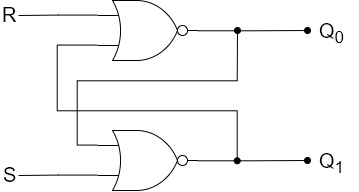
\includegraphics[width=0.6\textwidth]{../EJ6/Recursos/latch_sr_with_gates}
    \caption{Circuito Latch SR con compuertas lógicas discretas.}
    \label{fig:latch_sr_with_gates_ex6}
\end{figure}


\subsubsection{Flip-Flop D}
La tabla de verdad que representa a un Flip-Flop D es, por el contrario, la de la tabla \ref{table:ffd_truth_table_ex6}.
Luego, el circuito de implementación es el de la figura \ref{fig:ffd_with_gates_ex6}.
La parte del circuito indicada como Edge detector cumple la función de ser un detector de flancos que habilitará al circuito unicamente durante el tiempo que lo permite 
el retardo de las compuertas NOT no ideales que lo conforman.

\begin{table}[H]
    \centering
    \begin{tabular}{cc|cc}
    \textbf{S}   & \textbf{R} & \textbf{Q} & \textbf{~Q} \\ \hline
    $\uparrow$   & 0          & 0          & 1           \\
    $\uparrow$   & 1          & 1          & 0           \\
    X            & X          & Q          & ~Q         
    \end{tabular}
    \caption{Tabla de verdad del Flip-Flp D.}
    \label{table:ffd_truth_table_ex6}
\end{table}

\begin{figure}[H]
    \centering
    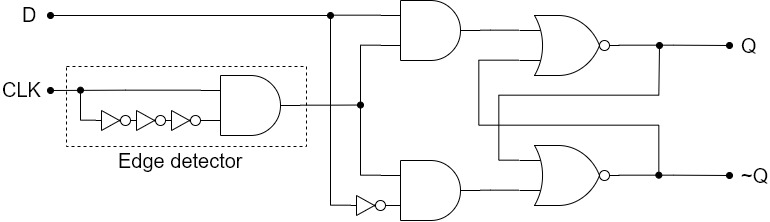
\includegraphics[width=0.8\textwidth]{../EJ6/Recursos/ffd_with_gates}
    \caption{Circuito Flip-Flop D con compuertas lógicas discretas.}
    \label{fig:ffd_with_gates_ex6}
\end{figure}



\subsection{Implementación en PCB}
Para la puesta en práctica de los circuitos mencionados en la sección anterior, se hace uso de dos placas.
La primera implementa el circuito de la figura \ref{fig:latch_sr_with_gates_ex6} utilizando el circuito integrado 74HCT02, el cual consta de 4 compuertas NOR de dos entradas. \\
La segunda se usa para implementar la primer etapa del circuito \ref{fig:ffd_with_gates_ex6} (hasta las salidas de las AND), y sus salidas se conectarán a la entrada 
de la primera placa para completar así el circuito de un Flip-Flop D.
Se emplean los integrados 74HCT02 para las compuertas NOT (cortocircuitando las entradas de las NOR), y 74HCT11, del cual se hacen uso de sus 3 compuertas AND de tres 
entradas, cortocircuitando dos de ellas.\\
Los esquemáticos resultantes son los de las figuras \ref{fig:latch_sr_schematic_ex6} y \ref{fig:ffd_adapter_schematic_ex6}.

\begin{figure}[H]
    \centering
    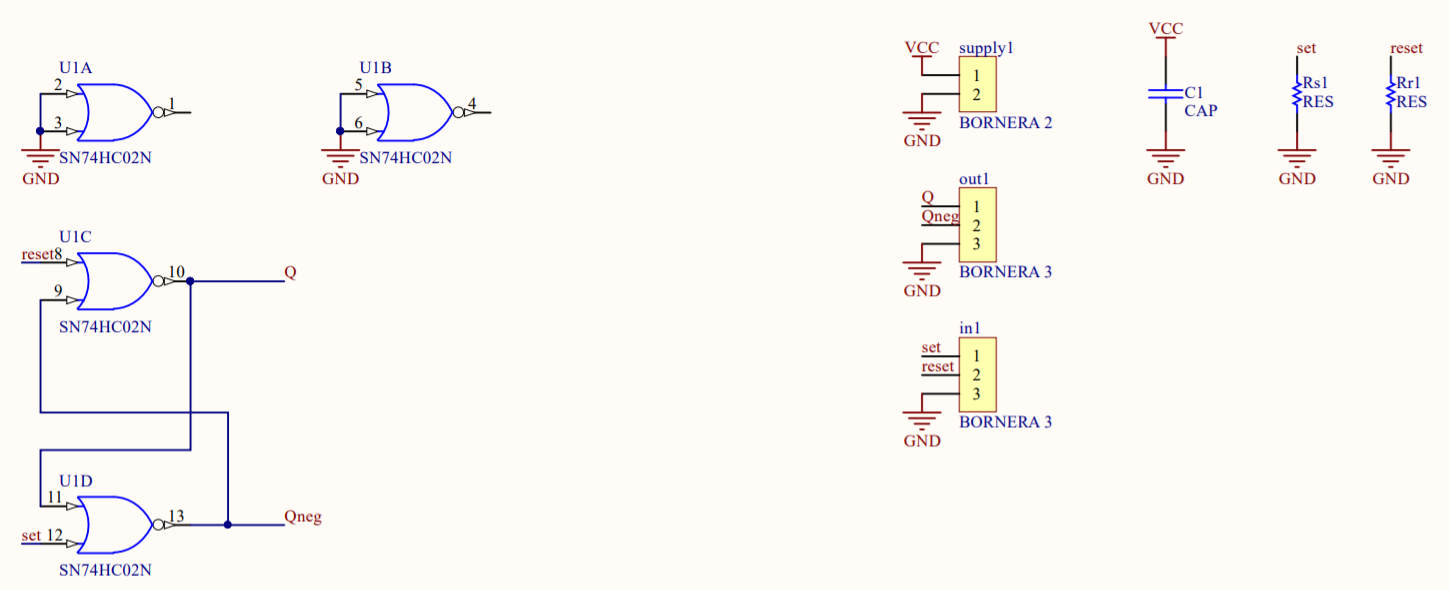
\includegraphics[width=0.8\textwidth]{../EJ6/Recursos/latch_sr_schematic}
    \caption{Esquemático para la placa del Latch SR.}
    \label{fig:latch_sr_schematic_ex6}
\end{figure}

\begin{figure}[H]
    \centering
    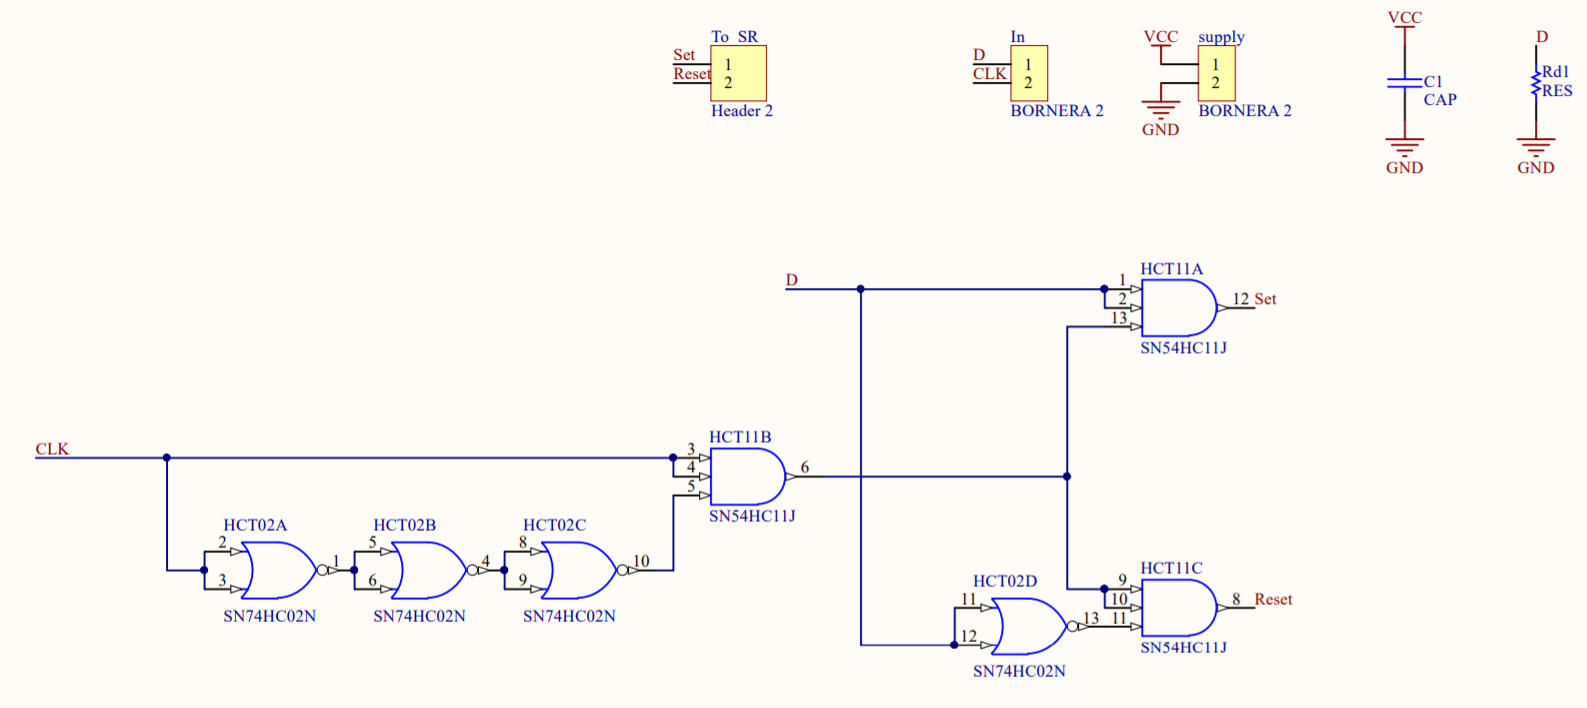
\includegraphics[width=0.8\textwidth]{../EJ6/Recursos/ffd_adapter_schematic}
    \caption{Esquemático para la placa de la entrada del Flip-Flop D.}
    \label{fig:ffd_adapter_schematic_ex6}
\end{figure}



\subsection{Medición de parámetros de los circuitos.}
A continuación se presentan todas las mediciones que se consideran necesarias para caracterizar a los circuitos implementados.
En ambos casos, se muestran, en primer lugar, mediciones cuyo objetivo es la observación cualitativa de la respuesta del sistema ante distintos estímulos, a fin de 
comprobar el correcto funcionamiento y el cumplimiento de las tablas de verdad para las que fueron diseñados.
Posteriormente, gráficos con un enfoque más concentrado en las transiciones son utilizados para comparar los tiempos de propagación, rise, fall, set up y hold, 
ofreciendo comparaciones con compuertas de uso comercial.


\subsubsection{Latch SR}
En primer lugar se verifica mediante las figuras \ref{fig:latch_sr_high_ex6} y \ref{fig:latch_sr_low_ex6} el correcto funcionamiento de las entradas set y reset, cumpliendo 
la función para la cual fueron diseñadas.
En la primera, mientras que la entrada de reset está conectada a 0V, se conecta una señal cuadrada al terminal de set, provocando que la salida sea un 1 lógico desde el 
primer momento en que set es también un 1, y este valor se mantiene luego cuando tanto set como reset son un 0 lógico.
El comportamiento opuesto se observa para la segunda figura, donde la señal de reset es la que está conectada a la entrada cuadrada, y set a masa, poniendo la salida en 0 
y manteniéndola en este valor.

\begin{figure}[H]
    \centering
    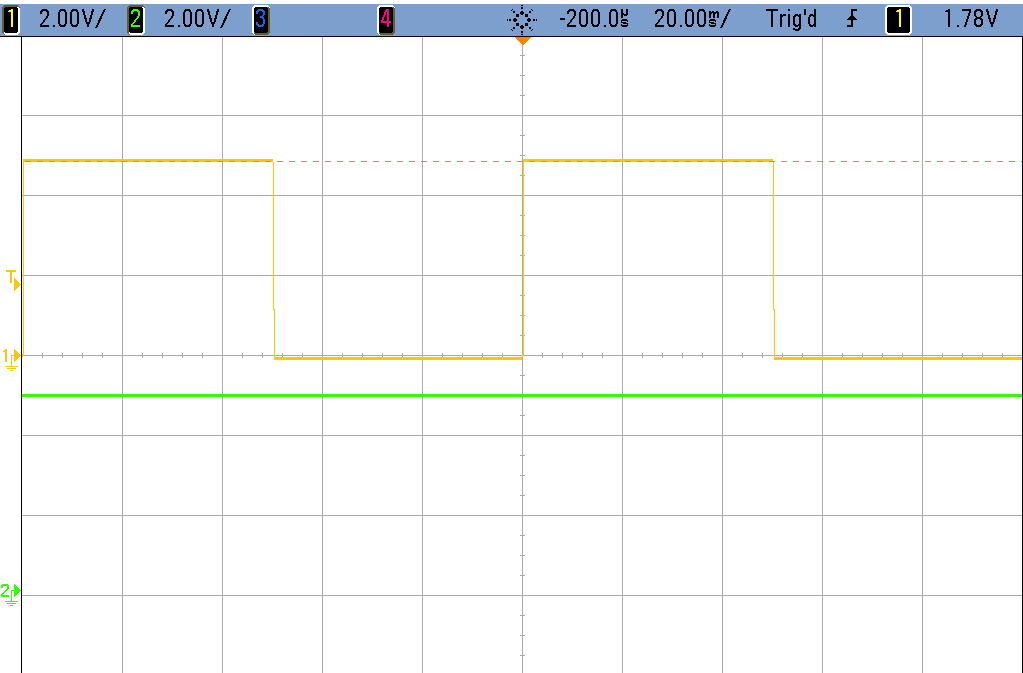
\includegraphics[width=0.6\textwidth]{../EJ6/Recursos/latch_sr_high}
    \caption{Latch SR con R en 0 y S alternando.}
    \label{fig:latch_sr_high_ex6}
\end{figure}

\begin{figure}[H]
    \centering
    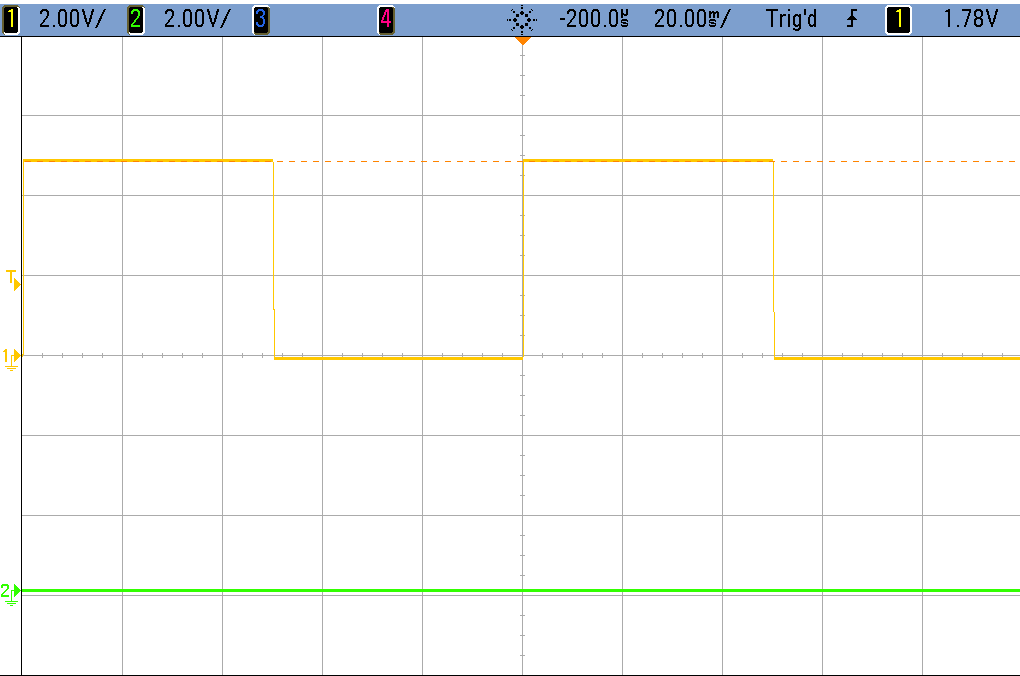
\includegraphics[width=0.6\textwidth]{../EJ6/Recursos/latch_sr_low}
    \caption{Latch SR con S en 0 y R alternando.}
    \label{fig:latch_sr_low_ex6}
\end{figure}

El análisis paramétrico del circuito se realiza observando las mediciones presentadas en las figuras \ref{fig:latch_sr_rise_ex6} y \ref{fig:latch_sr_fall_ex6}, 
extrayéndose de las mismas que los tiempos de rise y fall son de 5ns, y el de propagación, de 20ns.
Sin embargo, ha de considerarse que el tiempo de rise del osciloscopio, elemento de medición utilizado, es de $\frac{0,35}{fbw} = 3,5ns$ para $fbw = 100MHz$, con lo cual 
los tiempos de rise y fall medidos se encuentran cercanos al límite del aparato de medición; el valor medido puede, consecuentemente, acarrear un error producto de esto.
De todas maneras, se puede afirmar que los tiempos medidos estarán en ese rango de magnitud.

\begin{figure}[H]
    \centering
    \begin{tabular}{c c}
        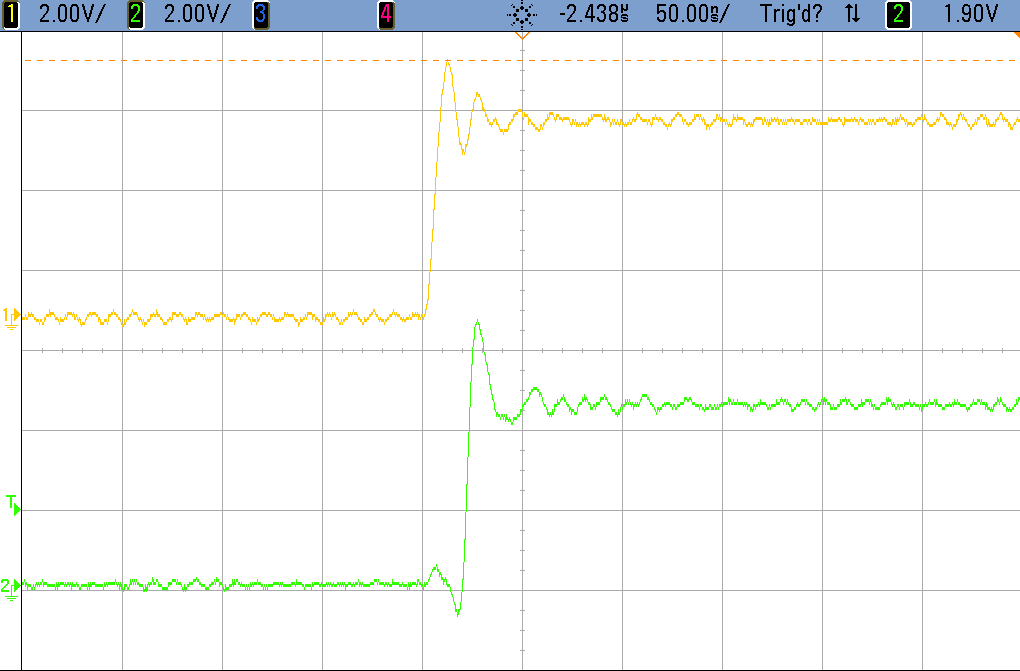
\includegraphics[width=0.5\textwidth]{../EJ6/Recursos/latch_sr_rise_osc} &
        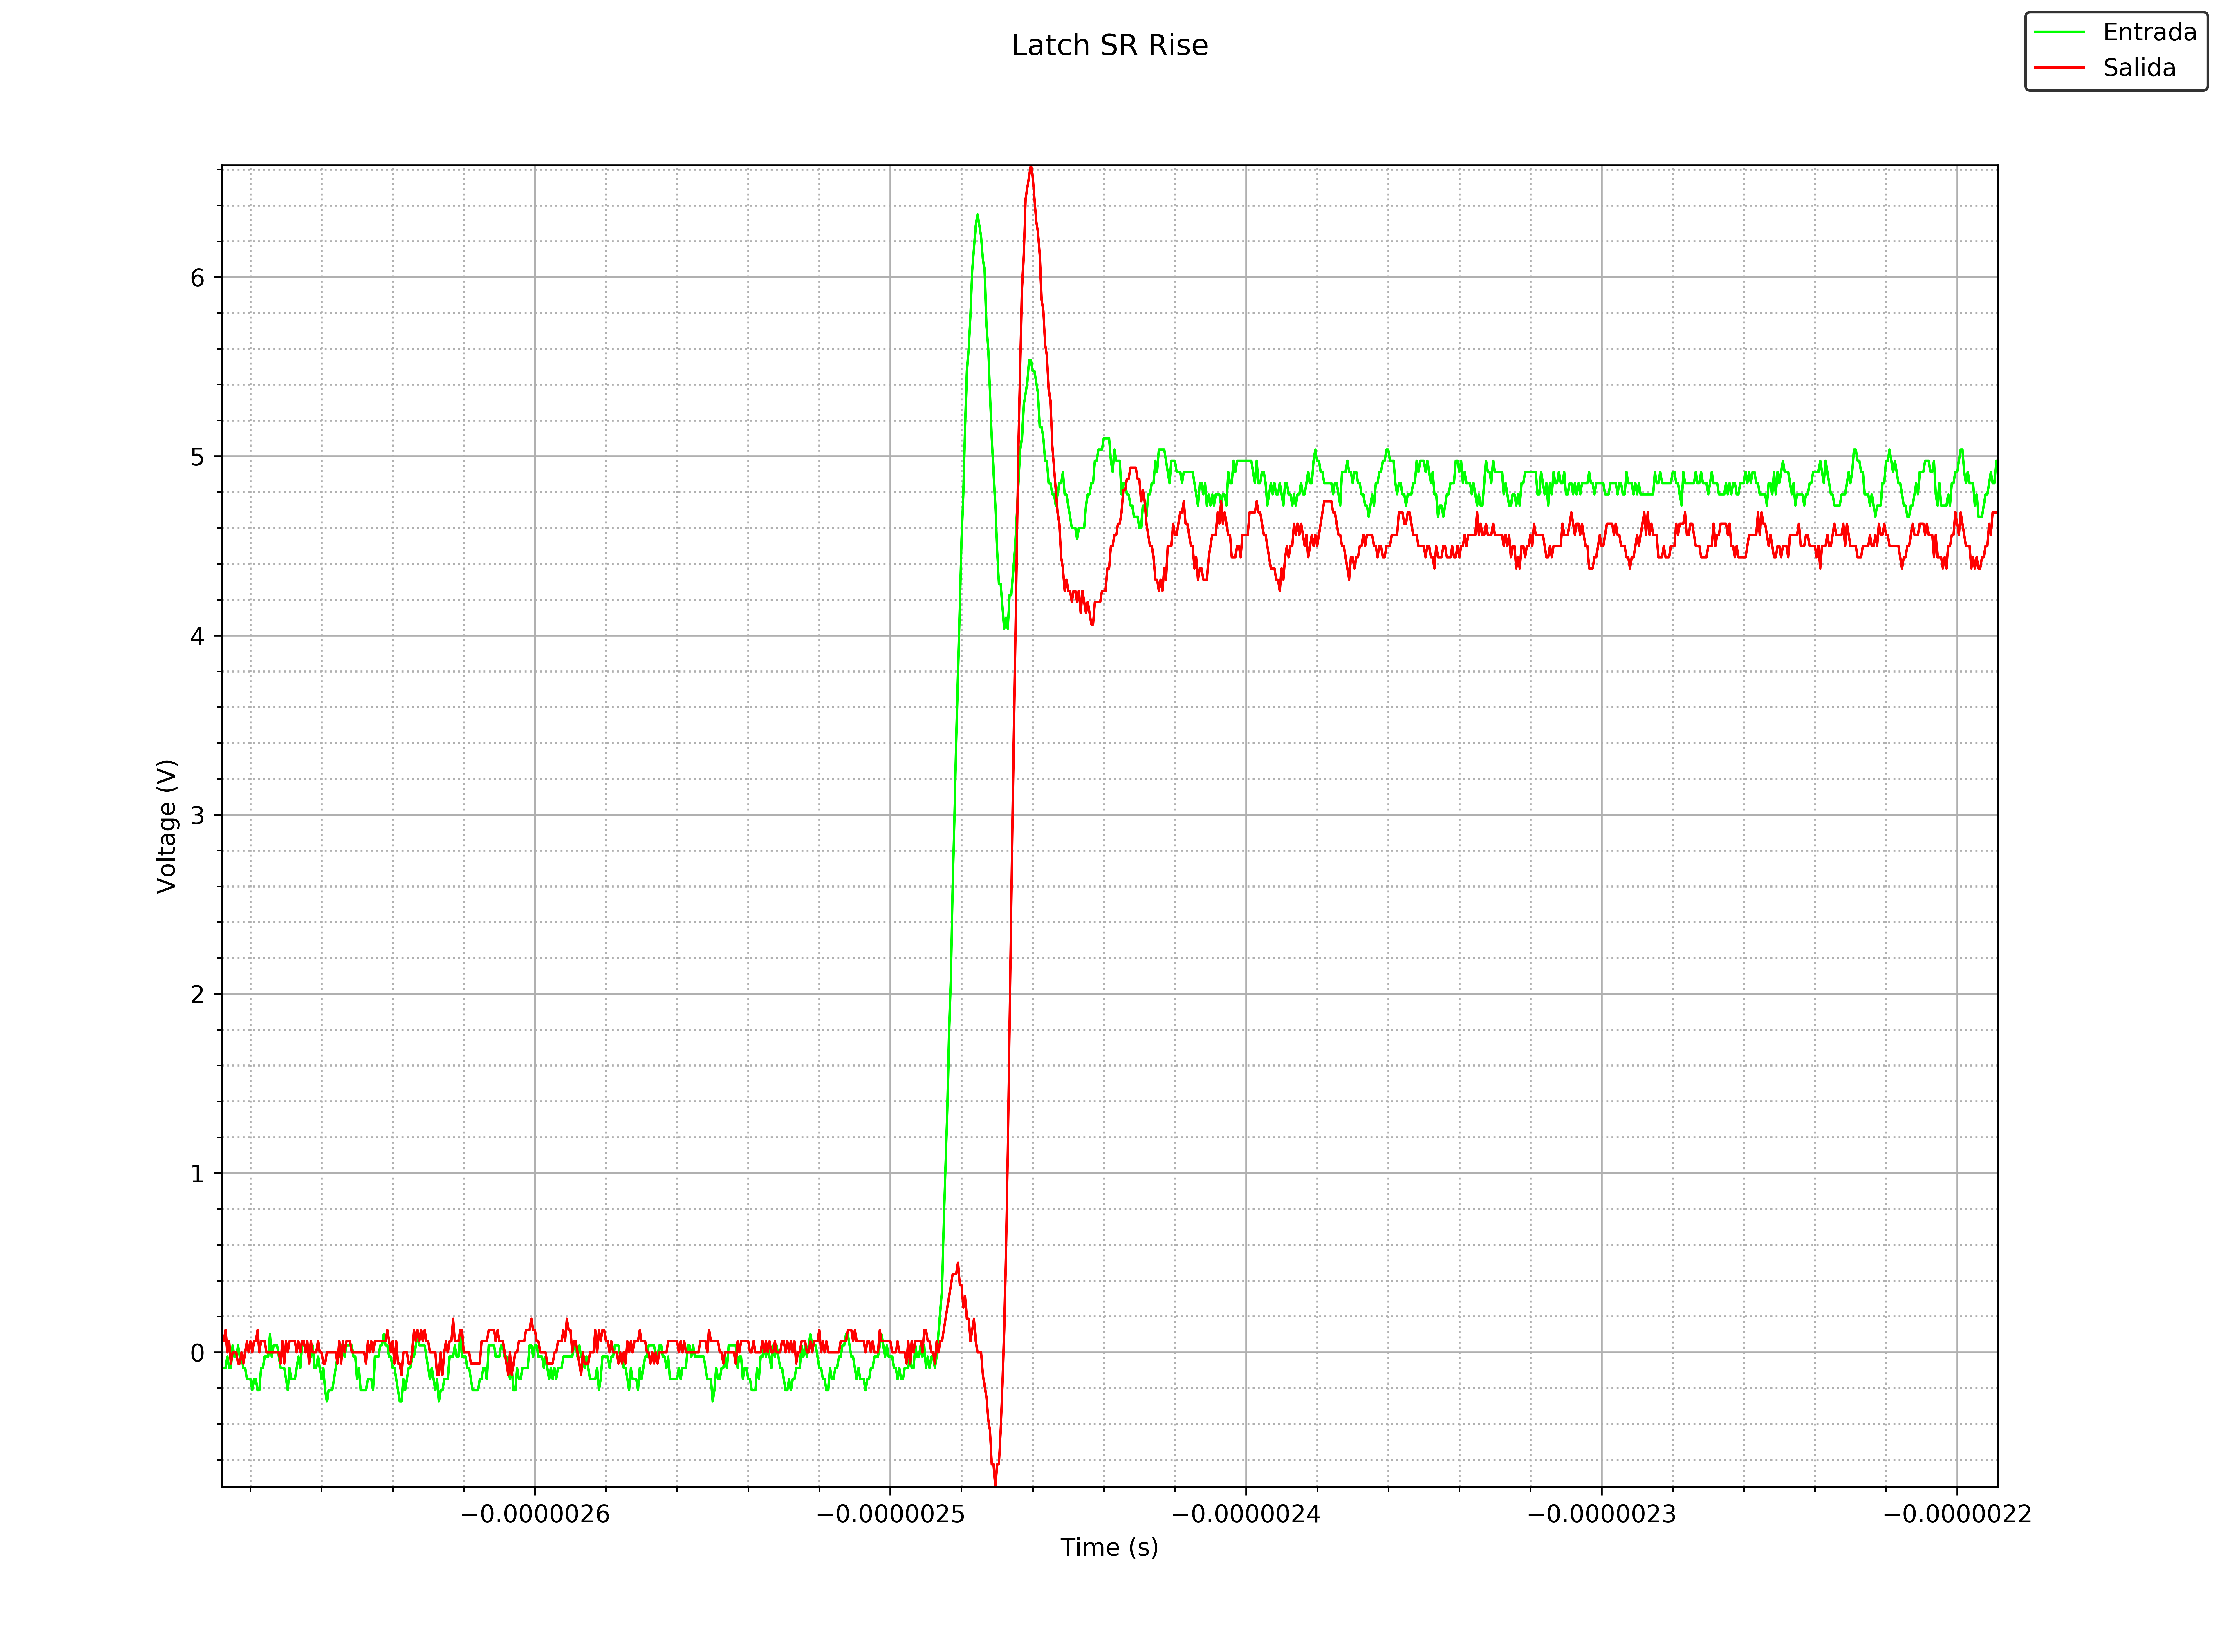
\includegraphics[width=0.5\textwidth]{../EJ6/Recursos/latch_sr_rise}
    \end{tabular}
    \caption{Transición del Latch SR de 0 a 1.}
    \label{fig:latch_sr_rise_ex6}
\end{figure}

\begin{figure}[H]
    \centering
    \begin{tabular}{c c}
        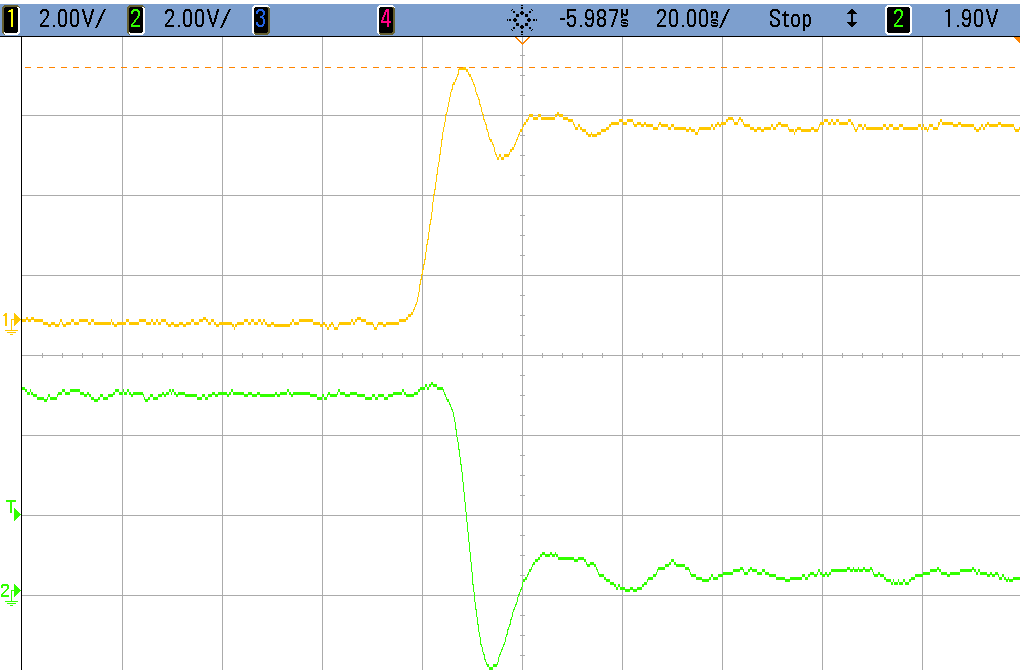
\includegraphics[width=0.5\textwidth]{../EJ6/Recursos/latch_sr_fall_osc} &
        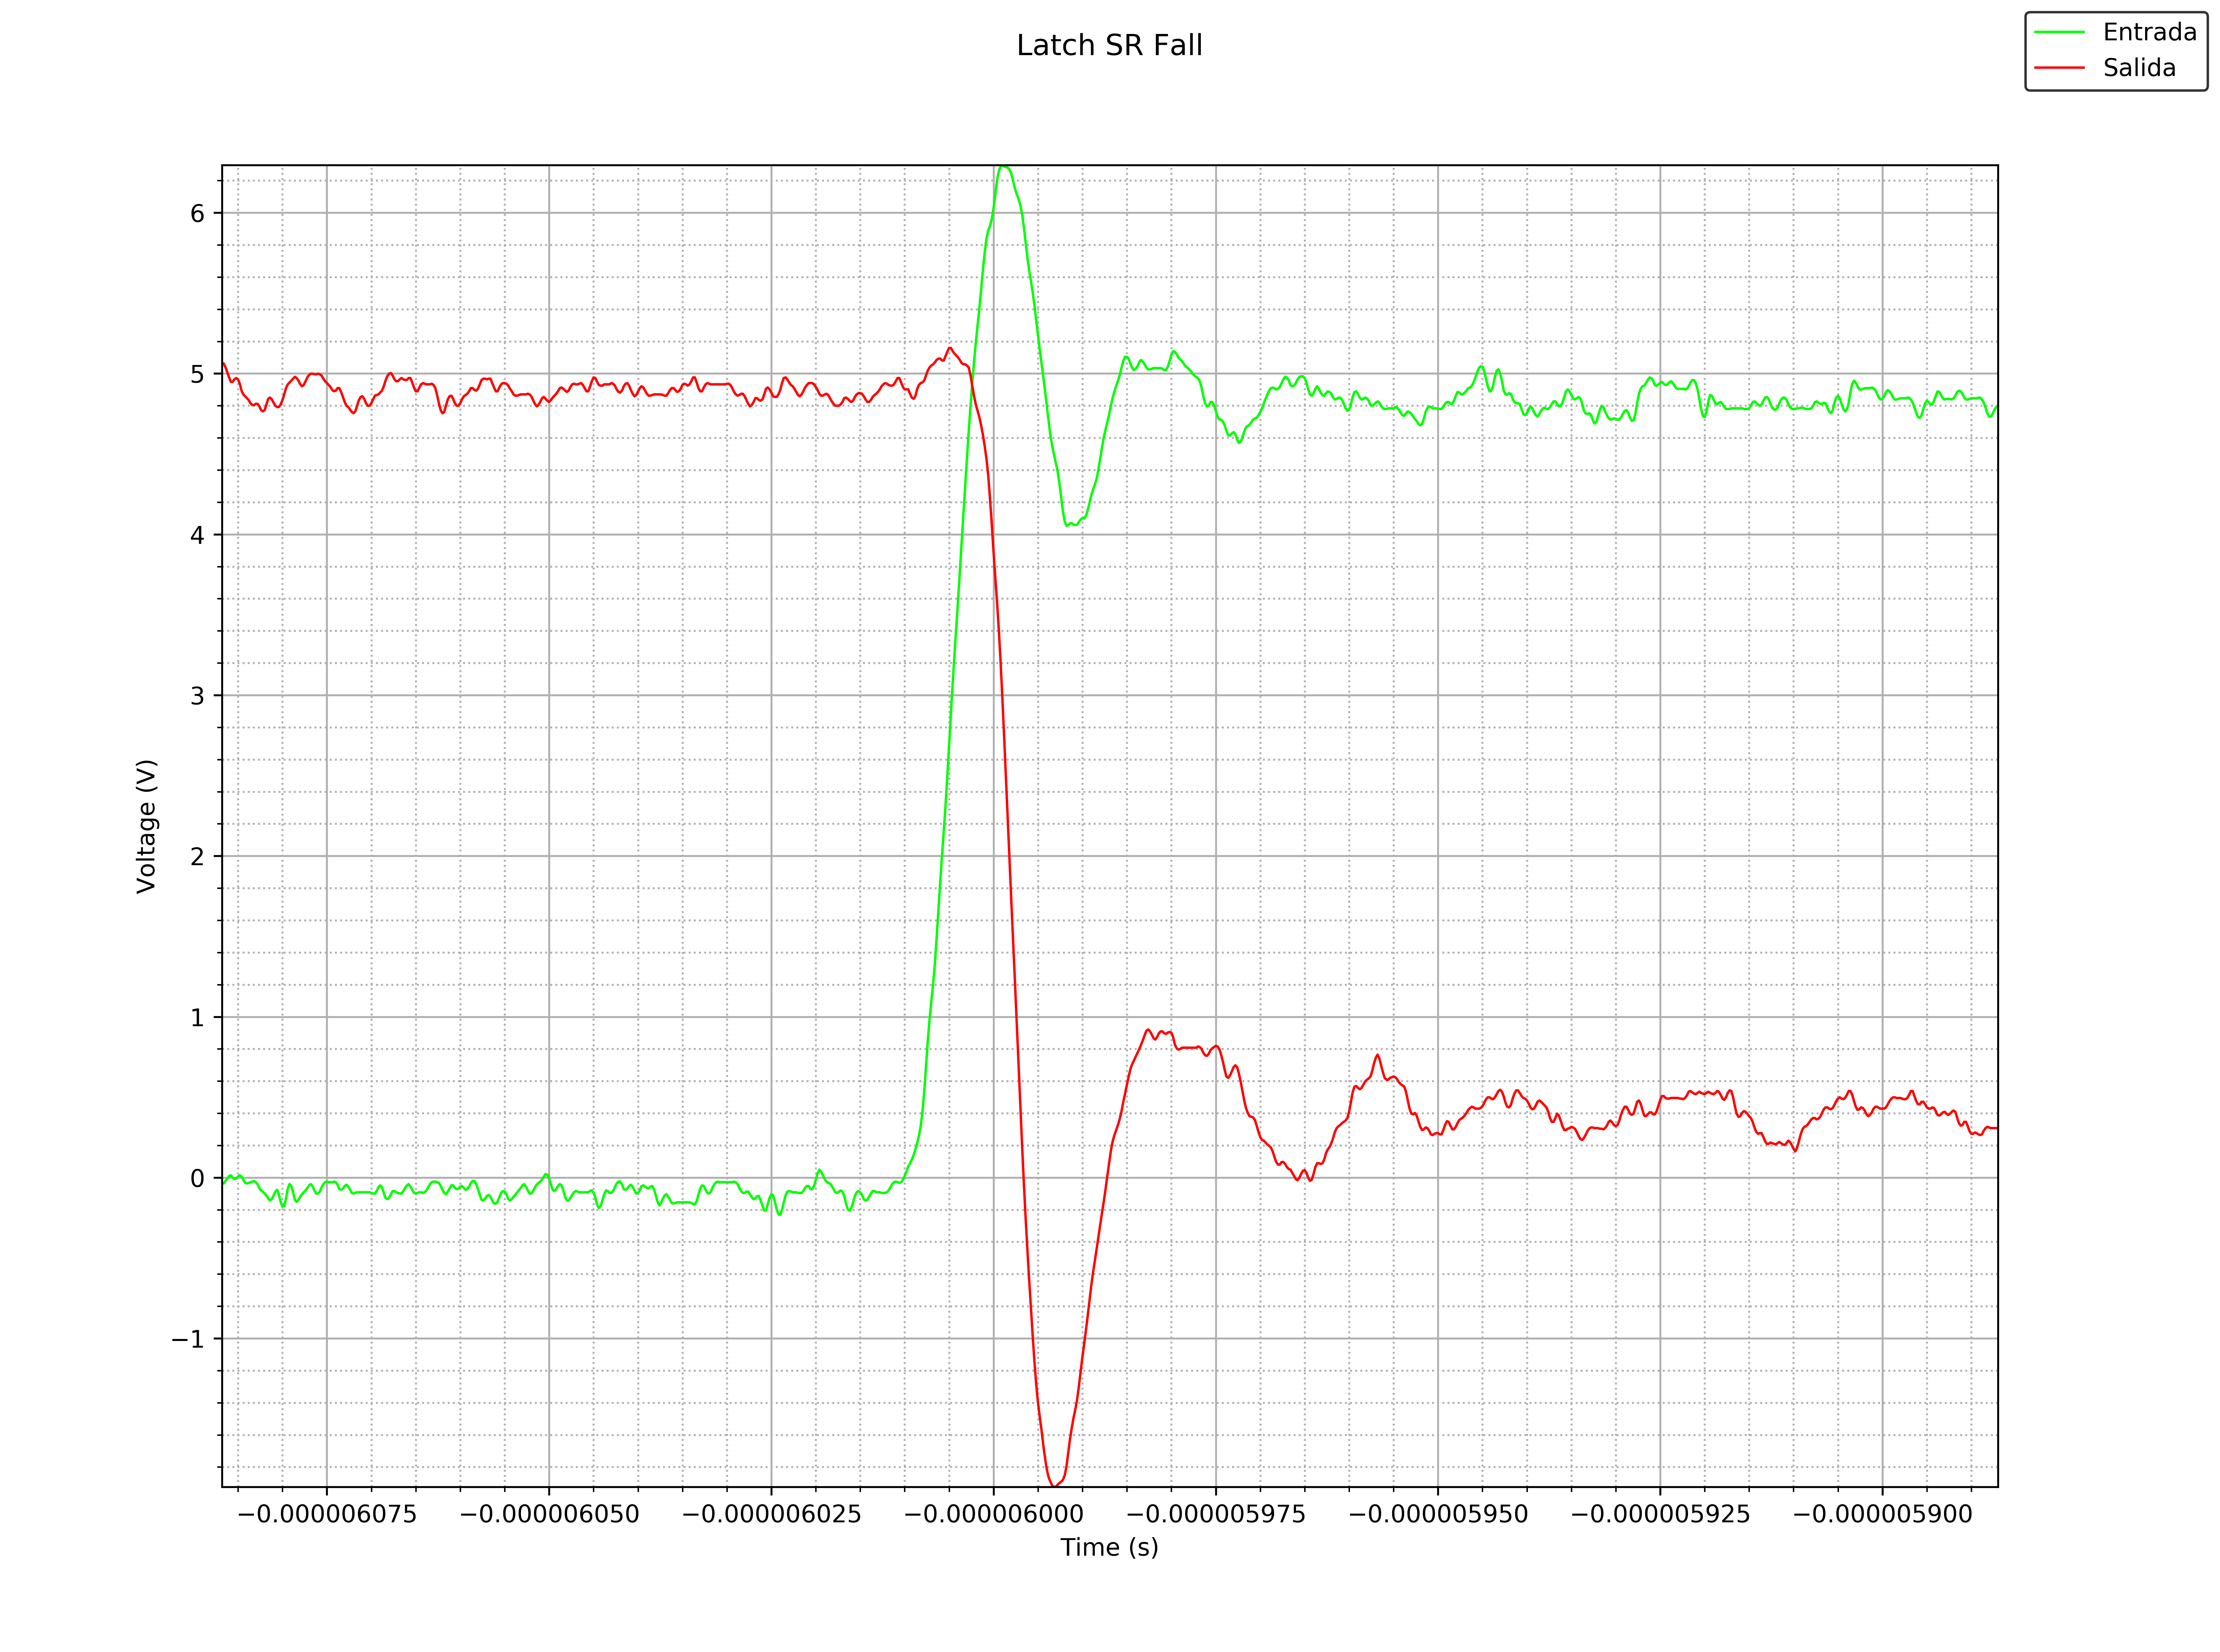
\includegraphics[width=0.5\textwidth]{../EJ6/Recursos/latch_sr_fall}
    \end{tabular}
    \caption{Transición del Latch SR de 1 a 0.}
    \label{fig:latch_sr_fall_ex6}
\end{figure}

La comparación con valores comerciales se hace mediante las figuras \ref{fig:com_latch_rise_ex6} y \ref{fig:com_latch_fall_ex6}, para las cuales se utilizó un Latch D 
ante la falta de disponibilidad de Latch SR comercial, y los resultados son similares a los de los circuitos hechos con compuertas lógicas.
Los tiempos de rise y fall parecen ser ligeramente menores para los componentes comerciales, aunque nuevamente debe remarcarse que se está midiendo cercano al límite del 
instrumento de medición.
La misma comparación se aplica para el tiempo de propagación, siendo este de 10ns aproximadamente.\\
Todas estas mediciones, además, se muestran en acuerdo con los datos en la datasheet del componente \footnote{https://assets.nexperia.com/documents/data-sheet/74HC\_HCT373.pdf}, 
donde se da un máximo de 18ns para los tiempos de rise y fall, y 45ns para el de propagación.

\begin{figure}[H]
    \centering
    \begin{tabular}{c c}
        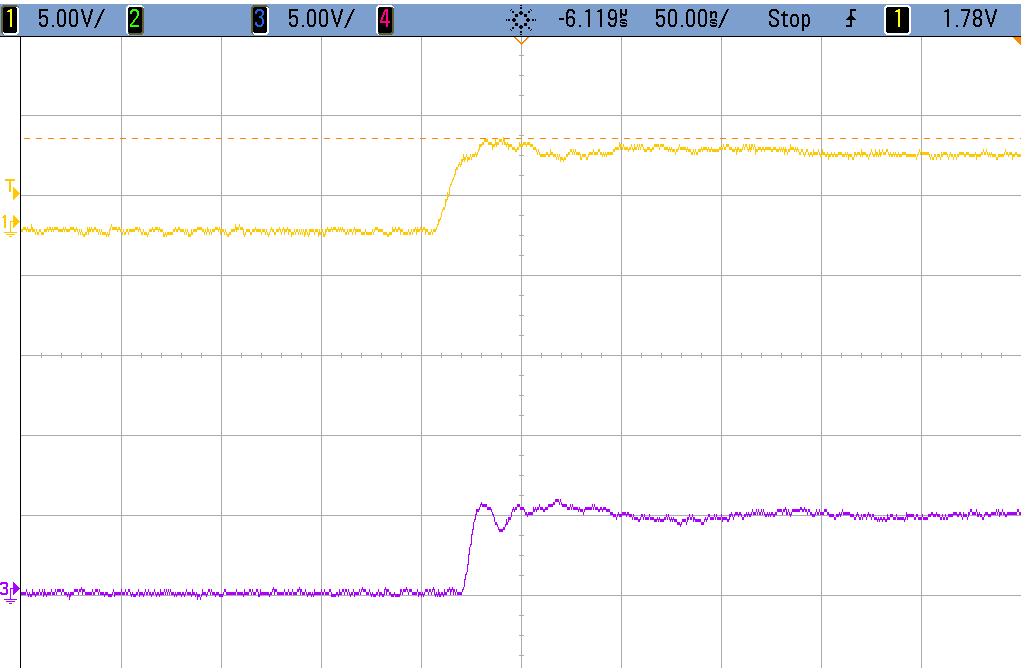
\includegraphics[width=0.5\textwidth]{../EJ6/Recursos/com_latch_rise_osc} &
        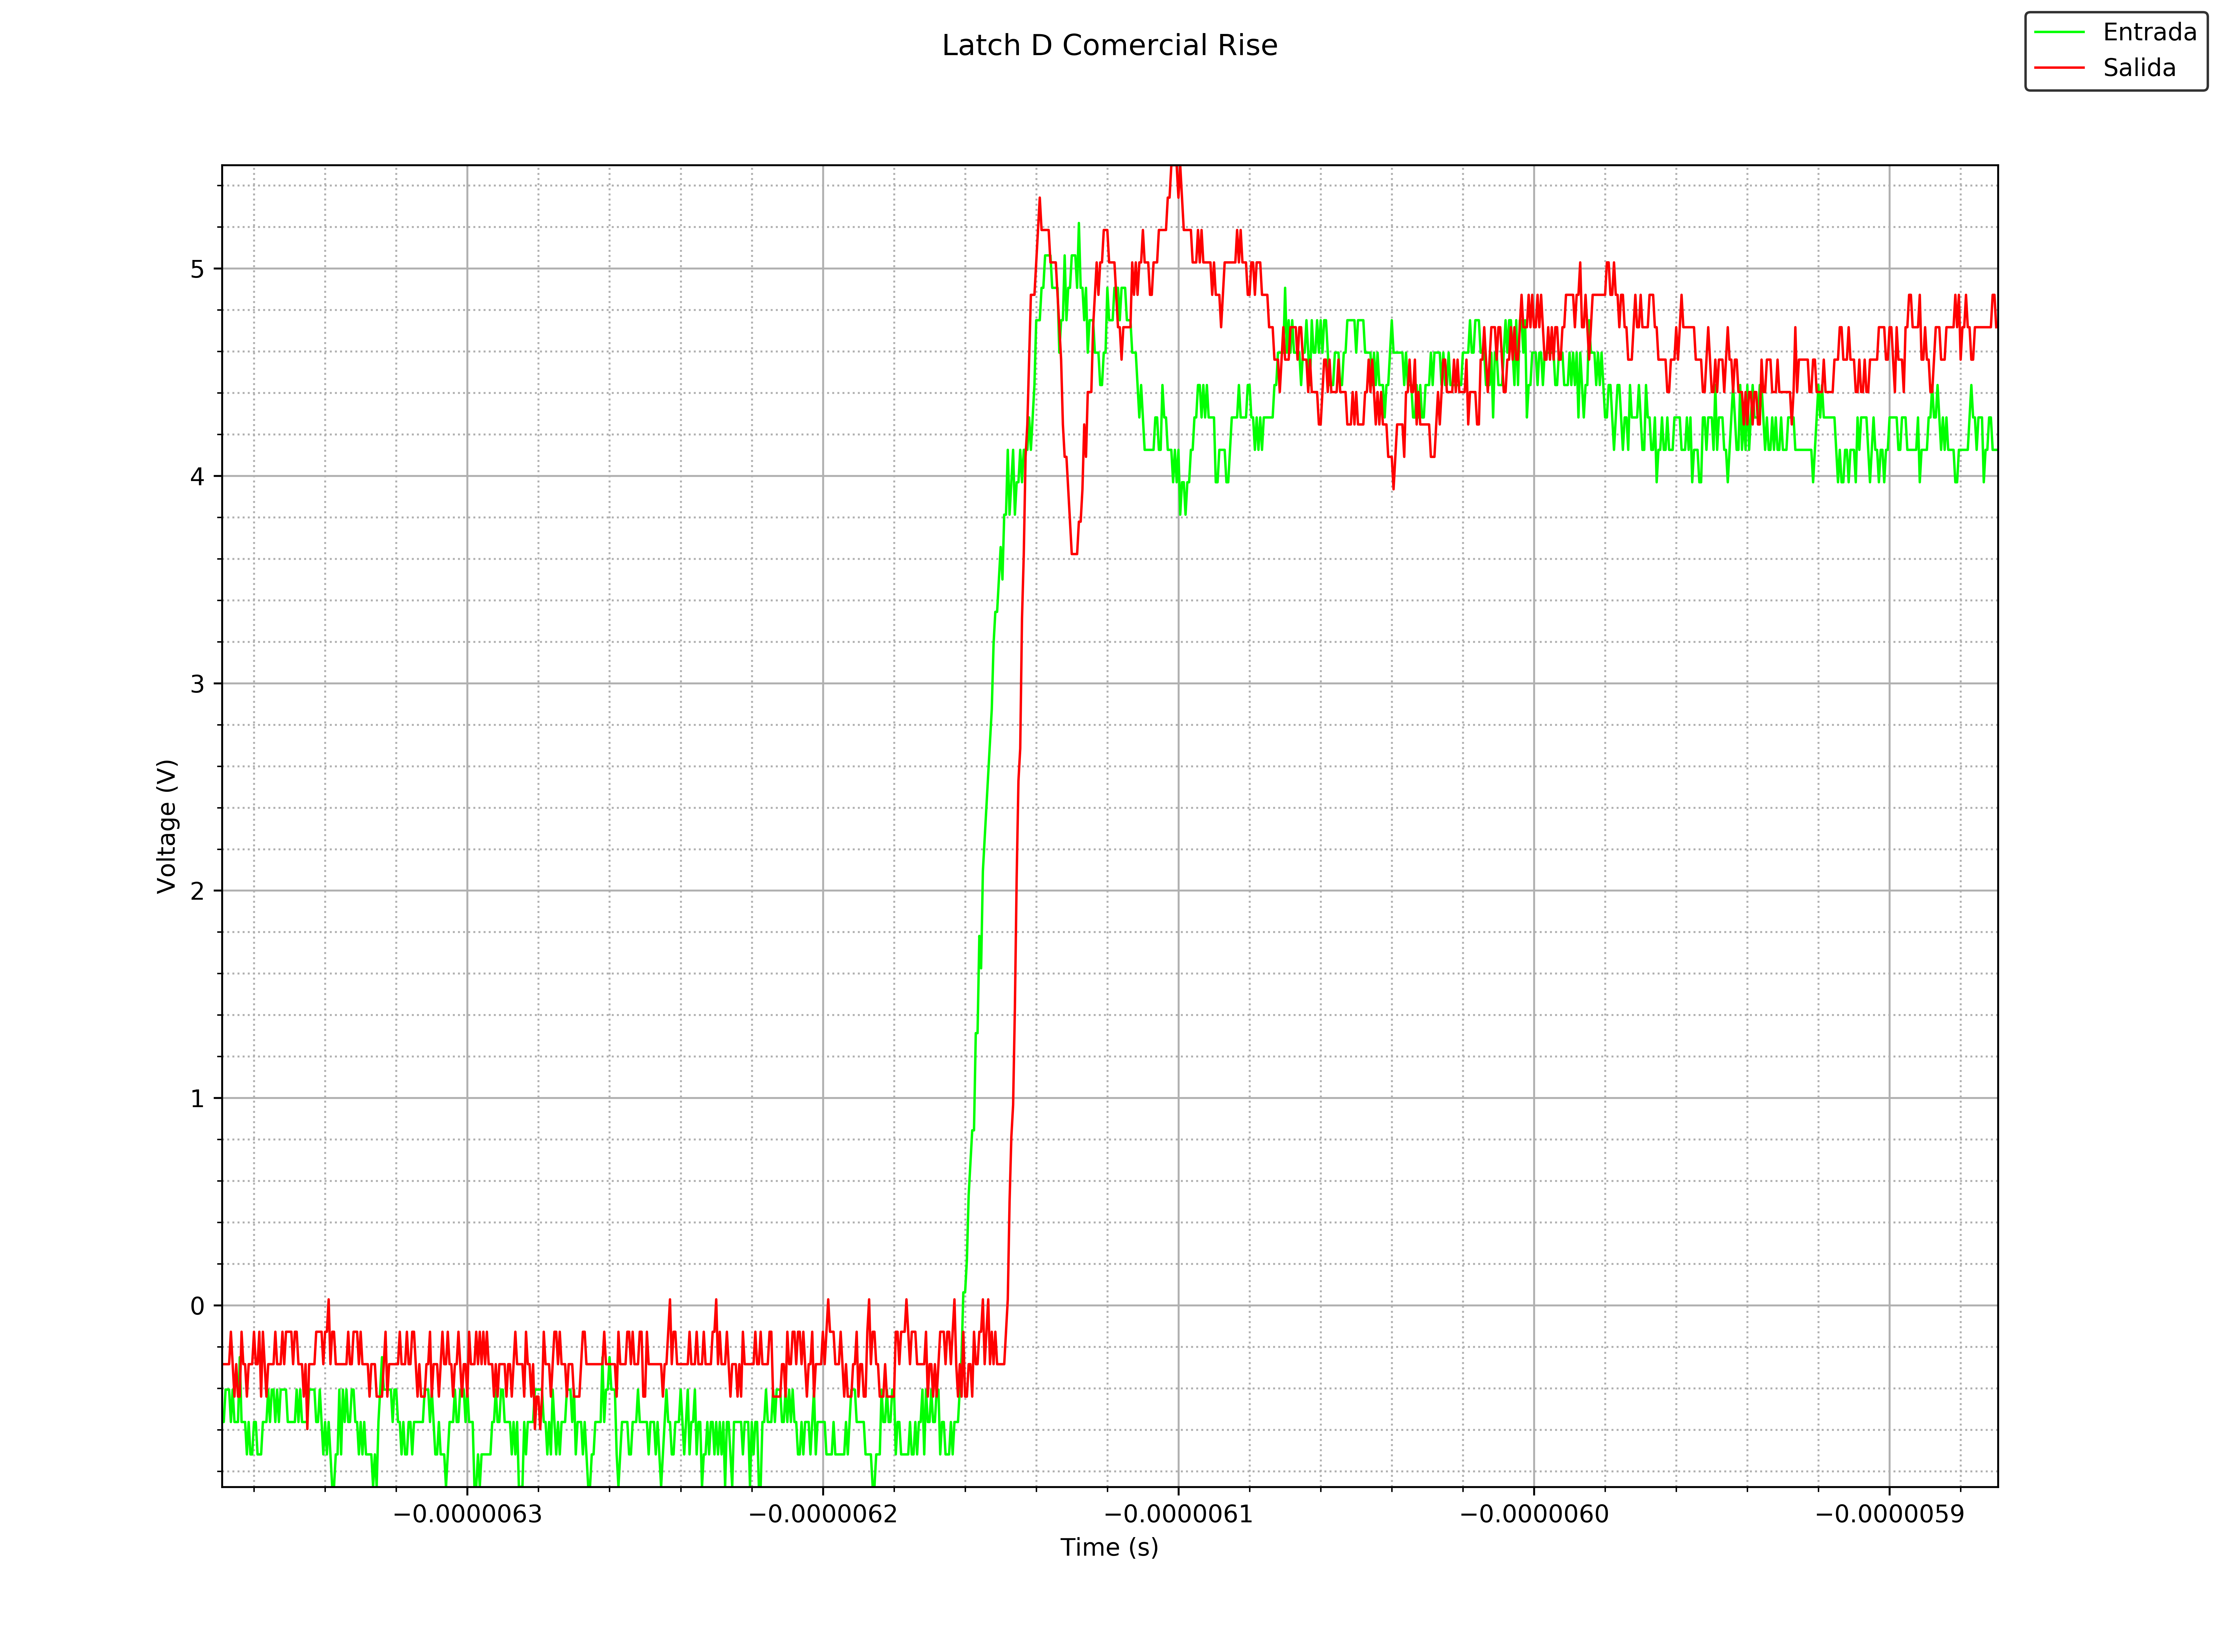
\includegraphics[width=0.5\textwidth]{../EJ6/Recursos/com_latch_rise}
    \end{tabular}
    \caption{Transición del Latch D comercial de 0 a 1.}
    \label{fig:com_latch_rise_ex6}
\end{figure}

\begin{figure}[H]
    \centering
    \begin{tabular}{c c}
        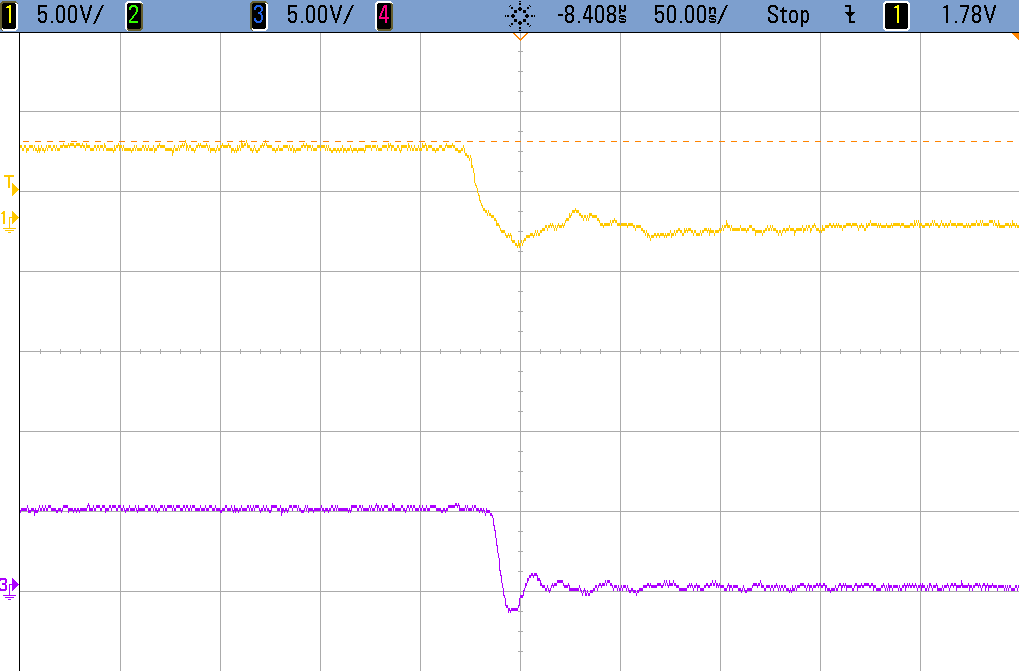
\includegraphics[width=0.5\textwidth]{../EJ6/Recursos/com_latch_fall_osc} &
        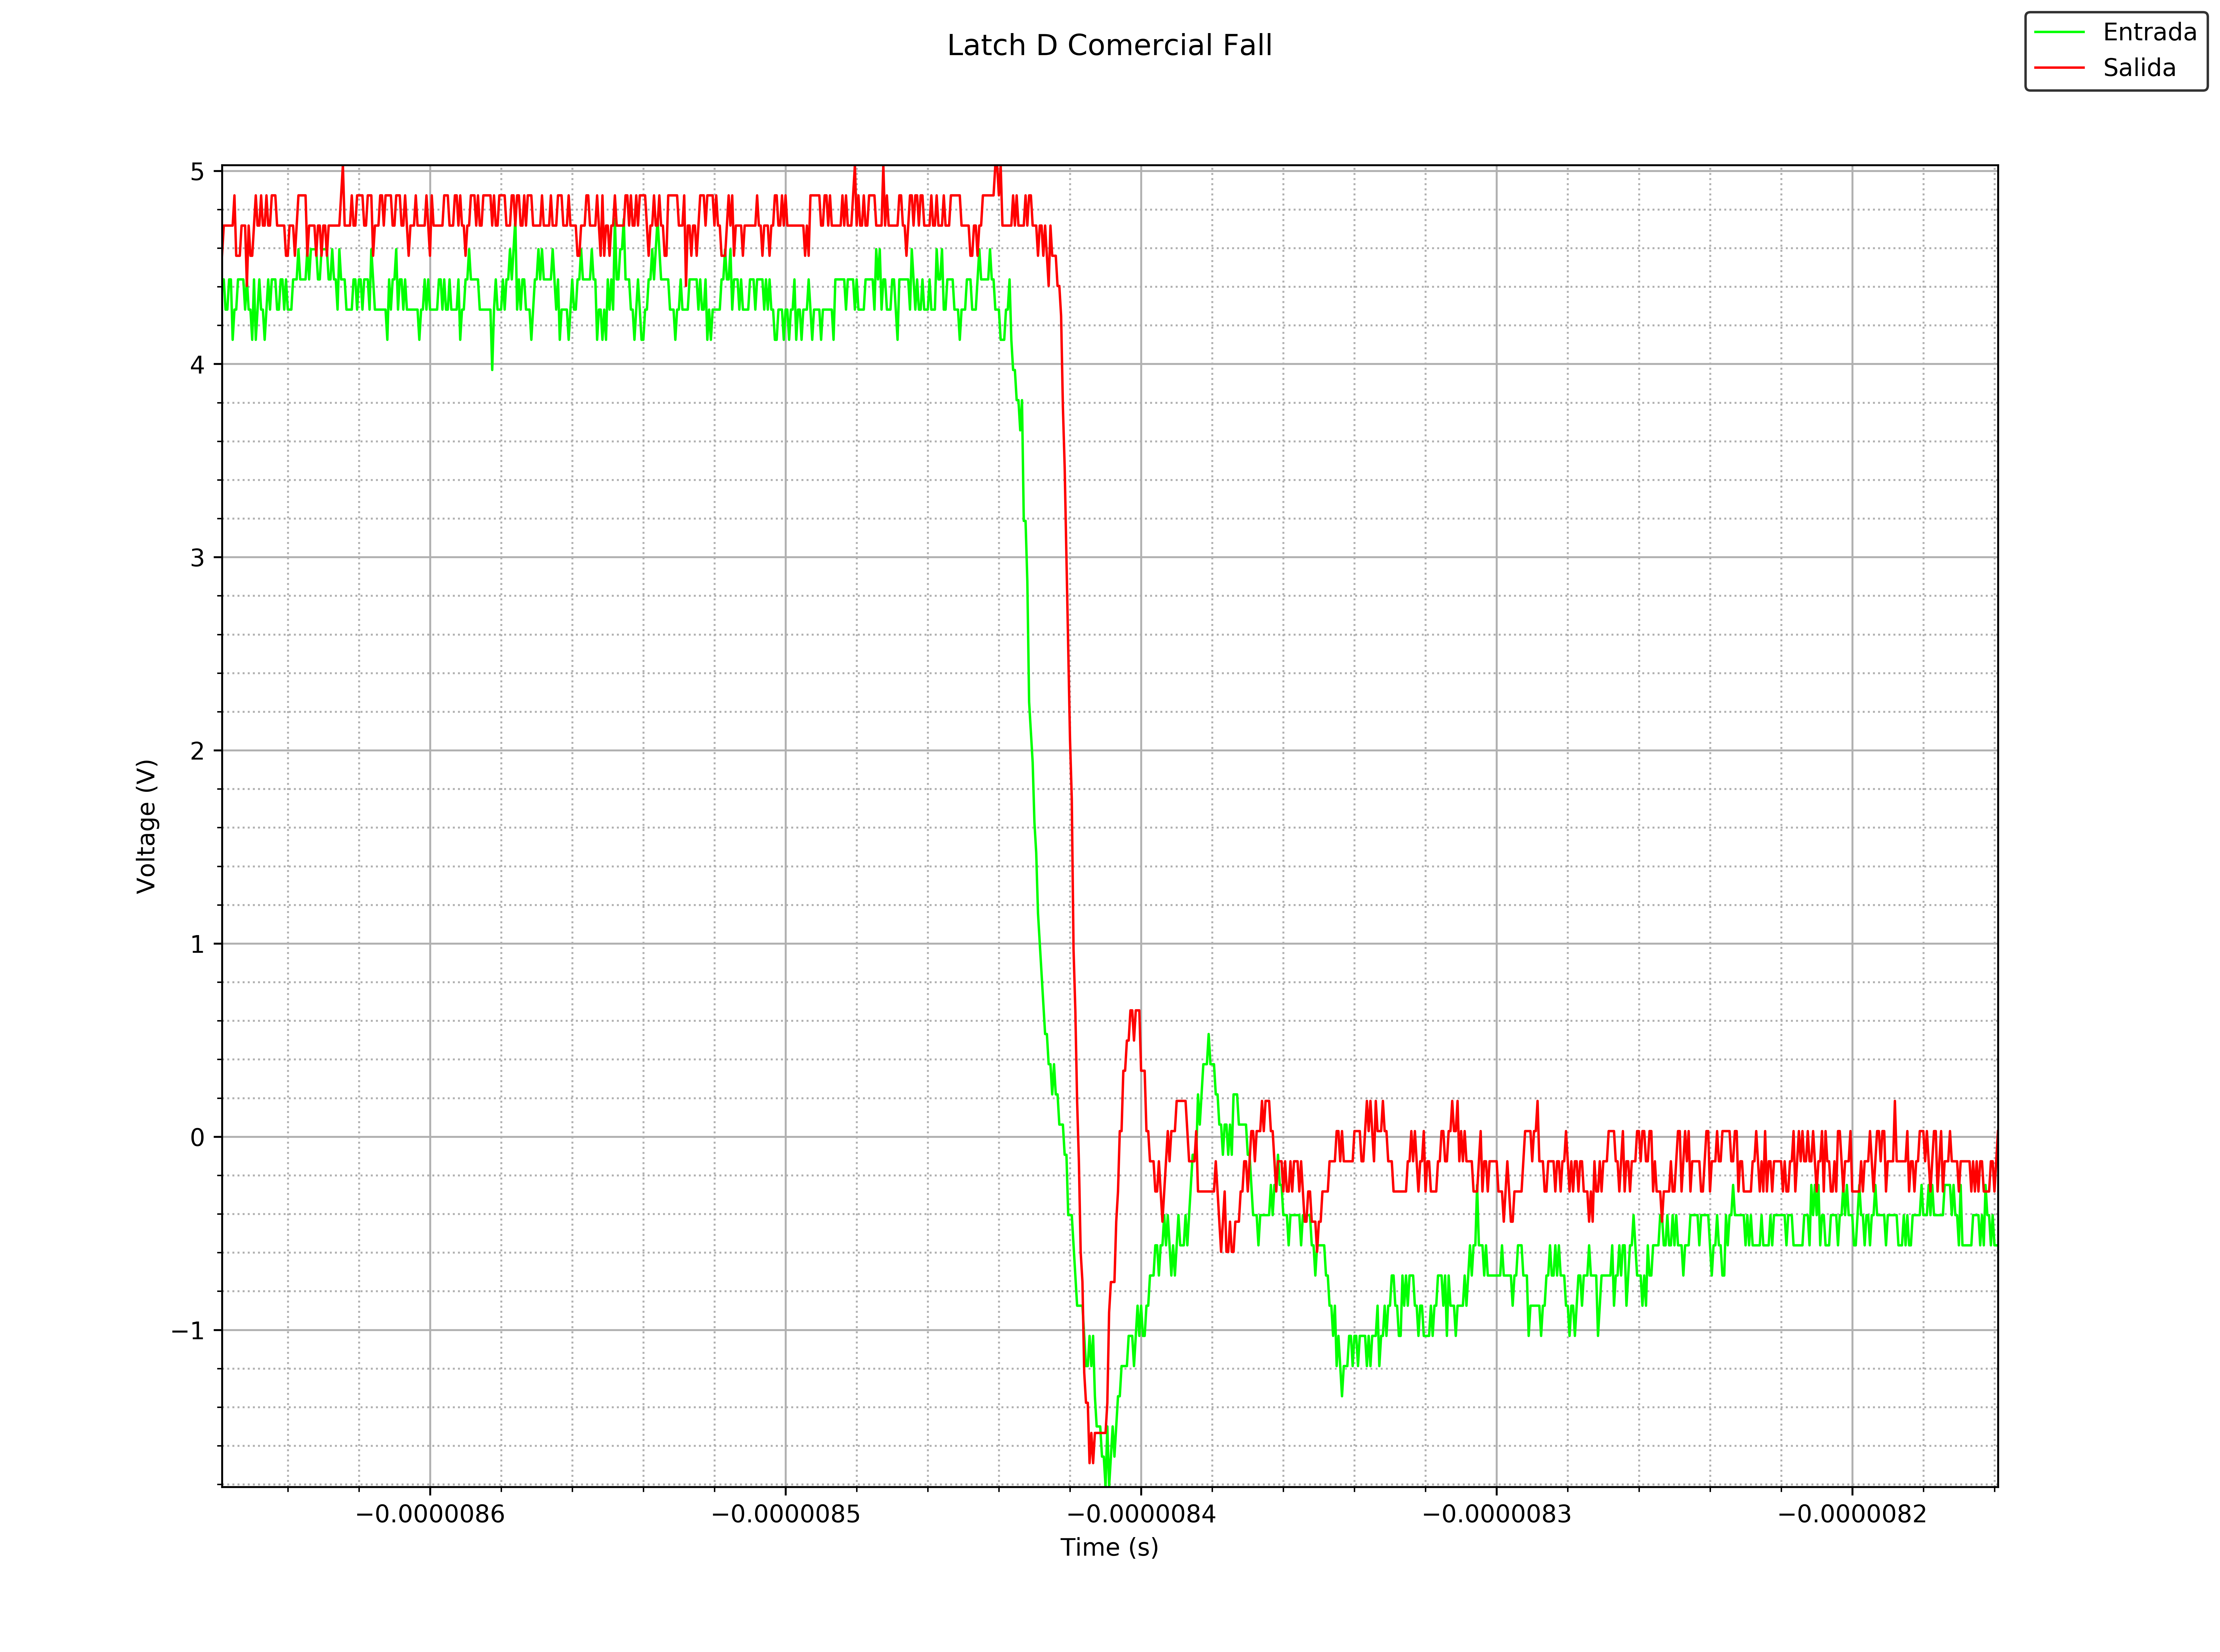
\includegraphics[width=0.5\textwidth]{../EJ6/Recursos/com_latch_fall}
    \end{tabular}
    \caption{Transición del Latch D comercial 1 a 0.}
    \label{fig:com_latch_fall_ex6}
\end{figure}

Finalmente, se considera pertinente remarcar el régimen transitorio de segundo orden que se observó en todas las mediciones, al cual puede asignársele una 
frecuencia característica.
Tanto para el componente comercial como para el circuito con compuertas, la frecuencia característica de la oscilación está en aproximadamente 33MHz, con no más de 3 
períodos de oscilación apreciable hasta la estabilización de la señal.


\subsubsection{Flip-Flop D}
De la misma manera que con el Latch, se corrobora el correcto funcionamiento del circuito a través de la figura \ref{fig:ffd_ex6}.
En ella se ve como, conforme a lo esperado, la salida en el tercer canal copia el valor de la entrada en el segundo canal, cuando se da un flanco ascendente del clock en 
el canal 1.

\begin{figure}[H]
    \centering
    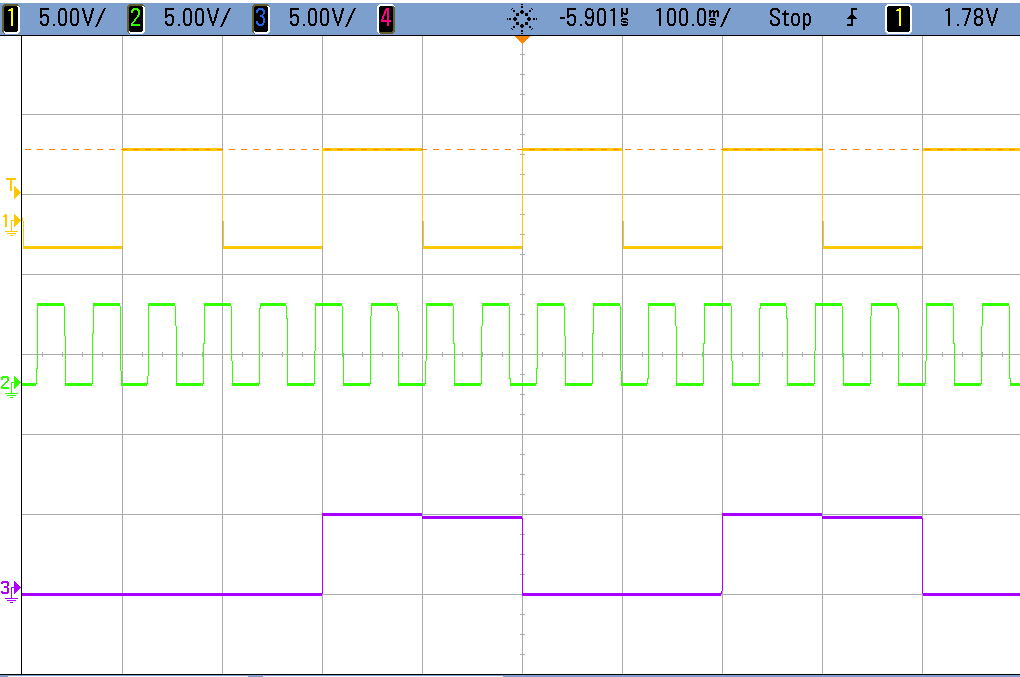
\includegraphics[width=0.6\textwidth]{../EJ6/Recursos/ffd_hold_and_set_up}
    \caption{Flip-Flop D, funcionamiento.}
    \label{fig:ffd_ex6}
\end{figure}

Los resultados de las mediciones de tiempo de rise y fall son análogos a los del Latch SR, mientras que el de propagación es de 40ns.
Esto último sigue el razonamiento lógico de que la acumulación de etapas de compuertas lógicas significará mayor tiempo de propagación.
Las mediciones pueden observarse en las figuras \ref{fig:ffd_rise_ex6} y \ref{fig:ffd_fall_ex6}.

\begin{figure}[H]
    \centering
    \begin{tabular}{c c}
        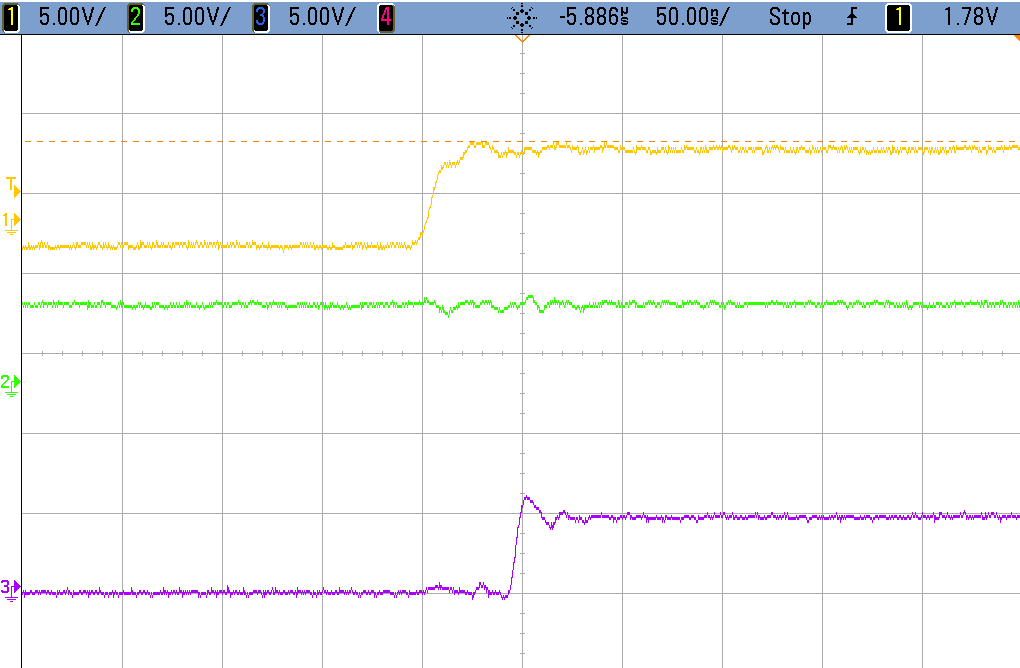
\includegraphics[width=0.5\textwidth]{../EJ6/Recursos/ffd_rise_osc} &
        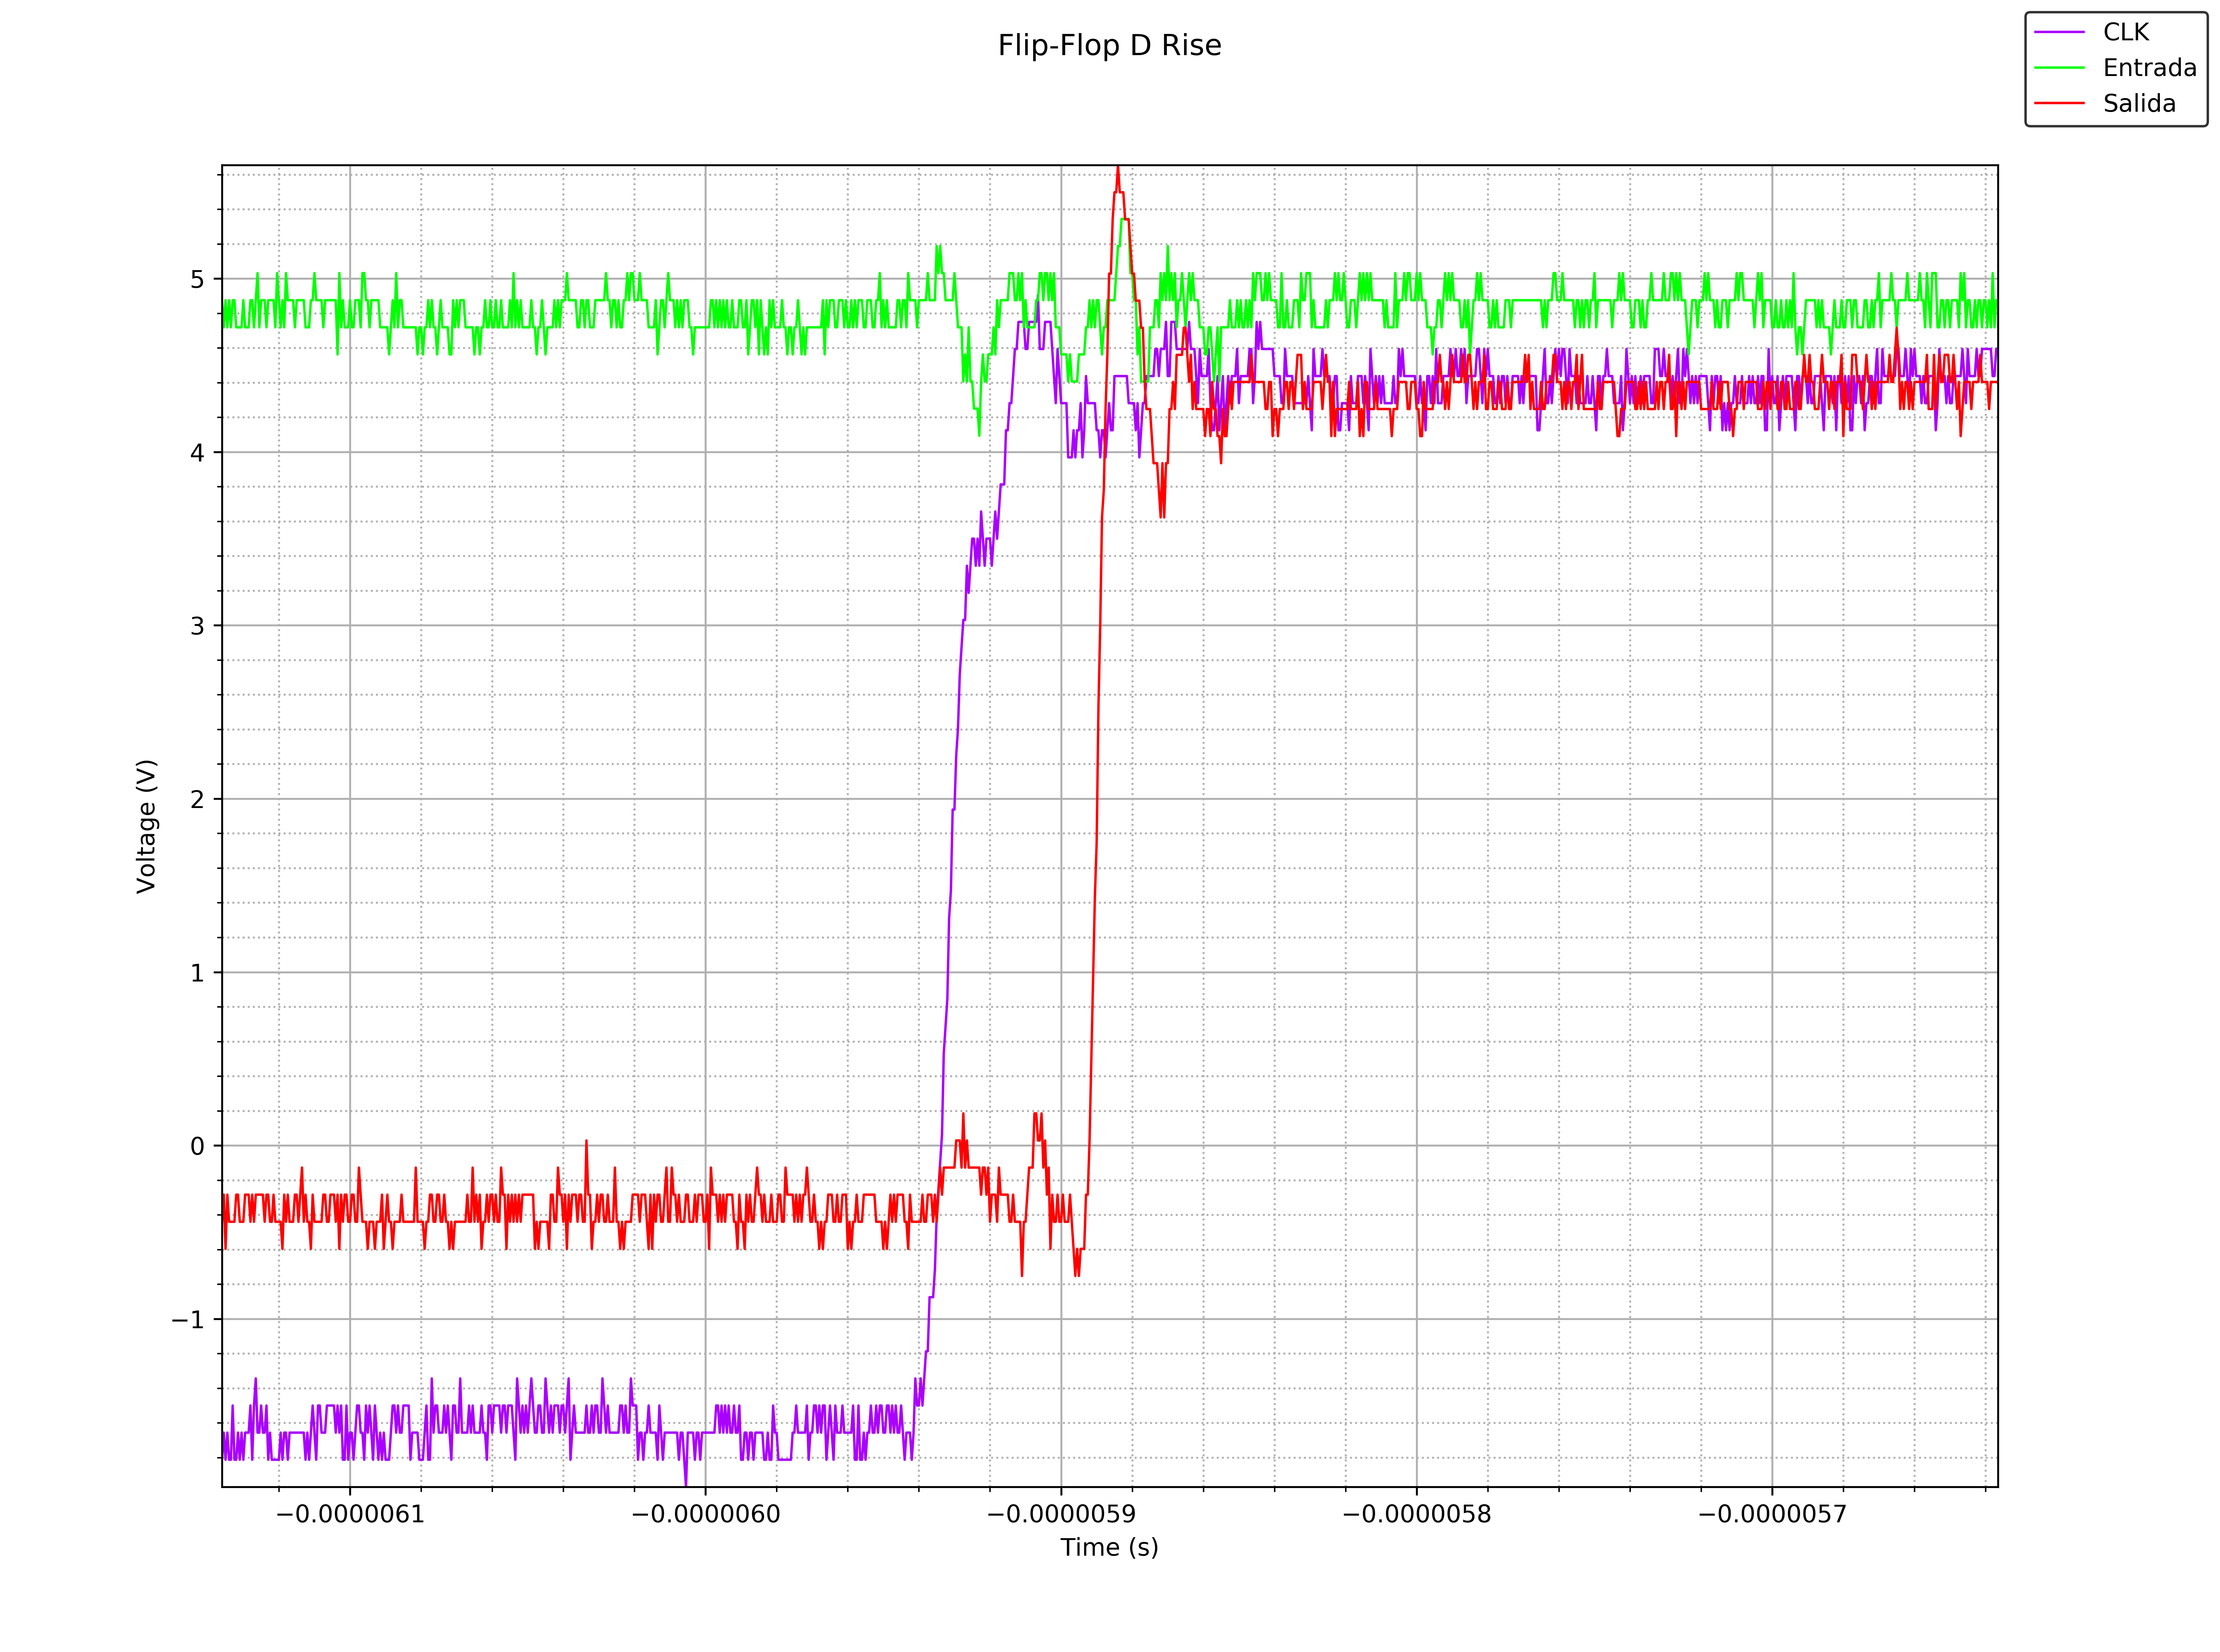
\includegraphics[width=0.5\textwidth]{../EJ6/Recursos/ffd_rise}
    \end{tabular}
    \caption{Transición del Flip-Flop D de 0 a 1.}
    \label{fig:ffd_rise_ex6}
\end{figure}

\begin{figure}[H]
    \centering
    \begin{tabular}{c c}
        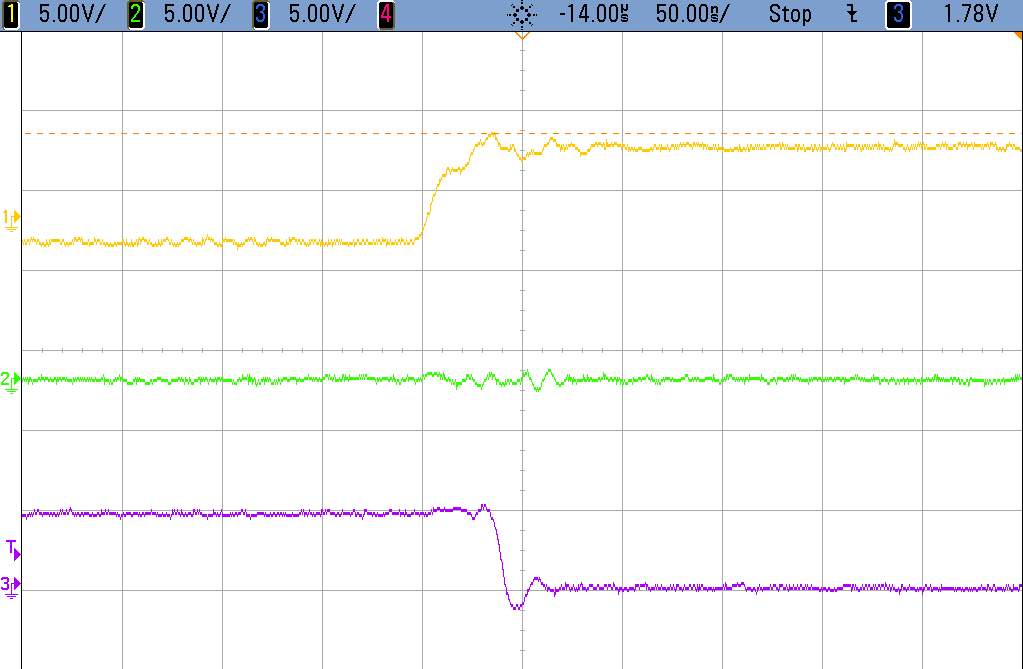
\includegraphics[width=0.5\textwidth]{../EJ6/Recursos/ffd_fall_osc} &
        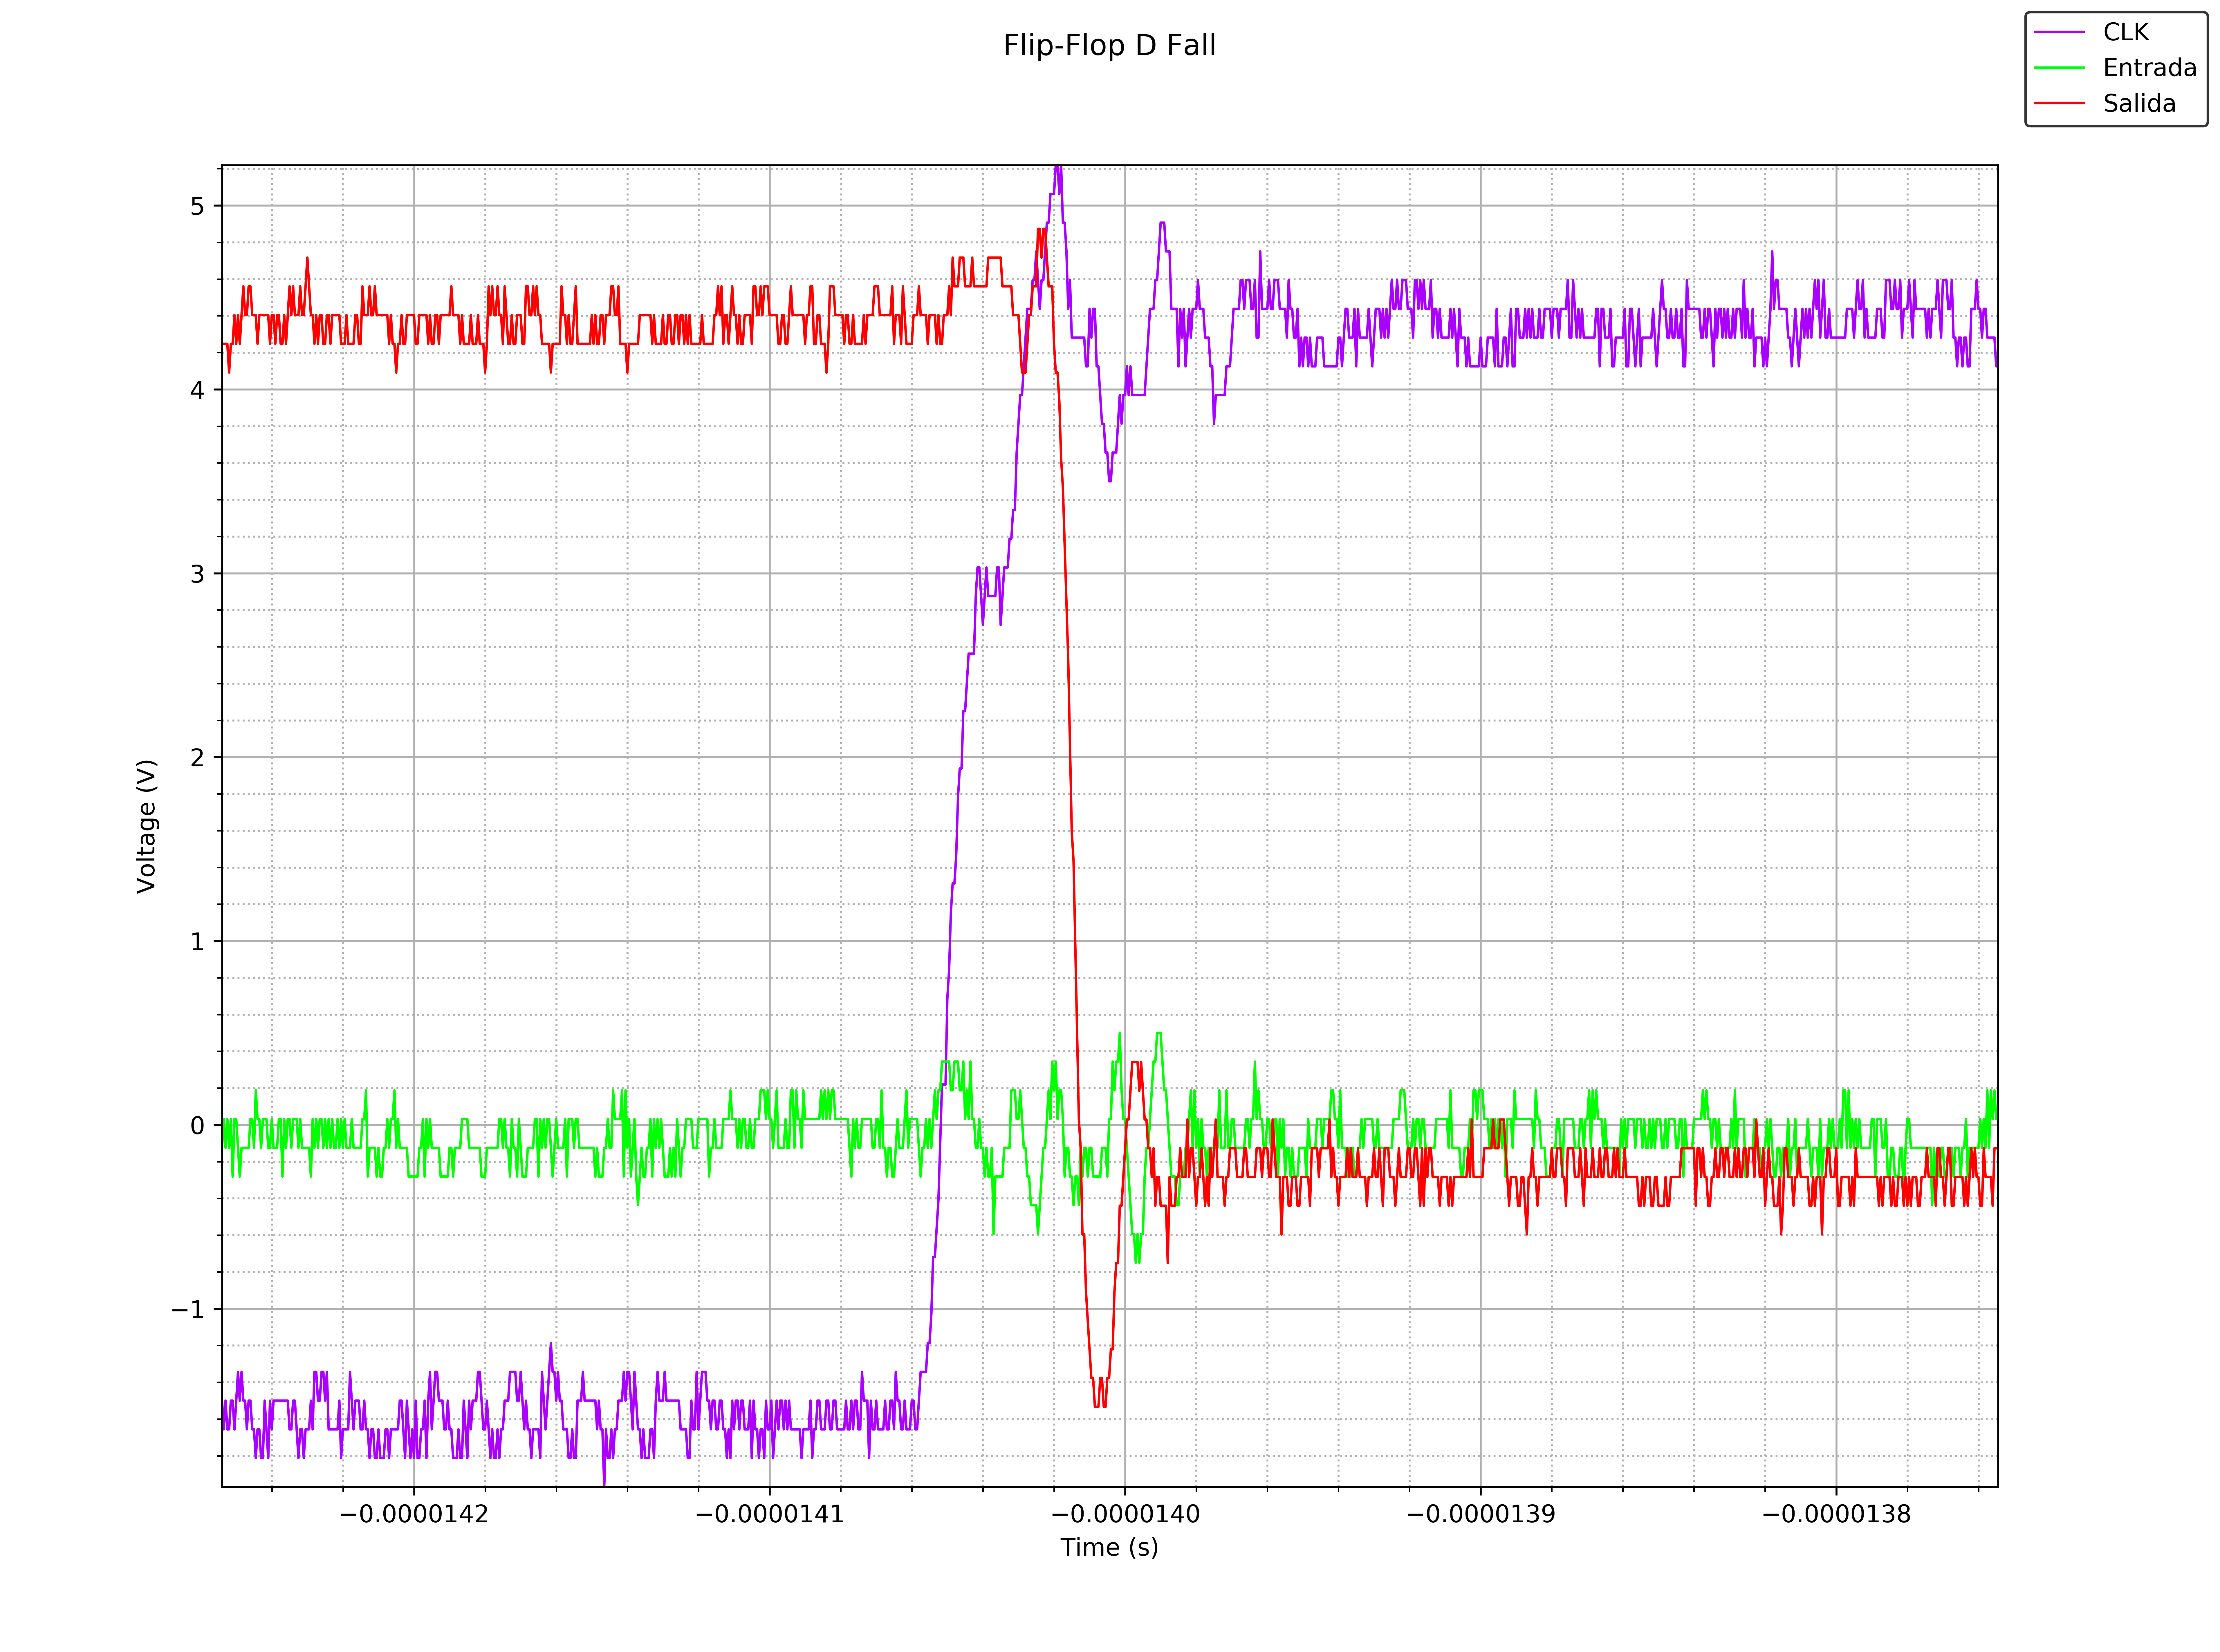
\includegraphics[width=0.5\textwidth]{../EJ6/Recursos/ffd_fall}
    \end{tabular}
    \caption{Transición del Flip-Flop D de 1 a 0.}
    \label{fig:ffd_fall_ex6}
\end{figure}

Es también análoga la comparación con componentes comerciales, donde además de repetirse que los tiempos de rise y fall están cercanos al límite de medición, se vuelve a 
dar que el tiempo de propagación se reduce a la mitad (20ns).\\
Nuevamente, todas estas mediciones se encuentran por debajo de los valores máximos especificados en datasheet\footnote{https://www.ti.com/lit/ds/schs183c/schs183c.pdf},
con tiempos de rise y fall menores a 15ns, y 41ns para el de propagación.
Para estos casos, las mediciones son las de las figuras \ref{fig:com_ffd_rise_ex6} y \ref{fig:com_ffd_fall_ex6}.

\begin{figure}[H]
    \centering
    \begin{tabular}{c c}
        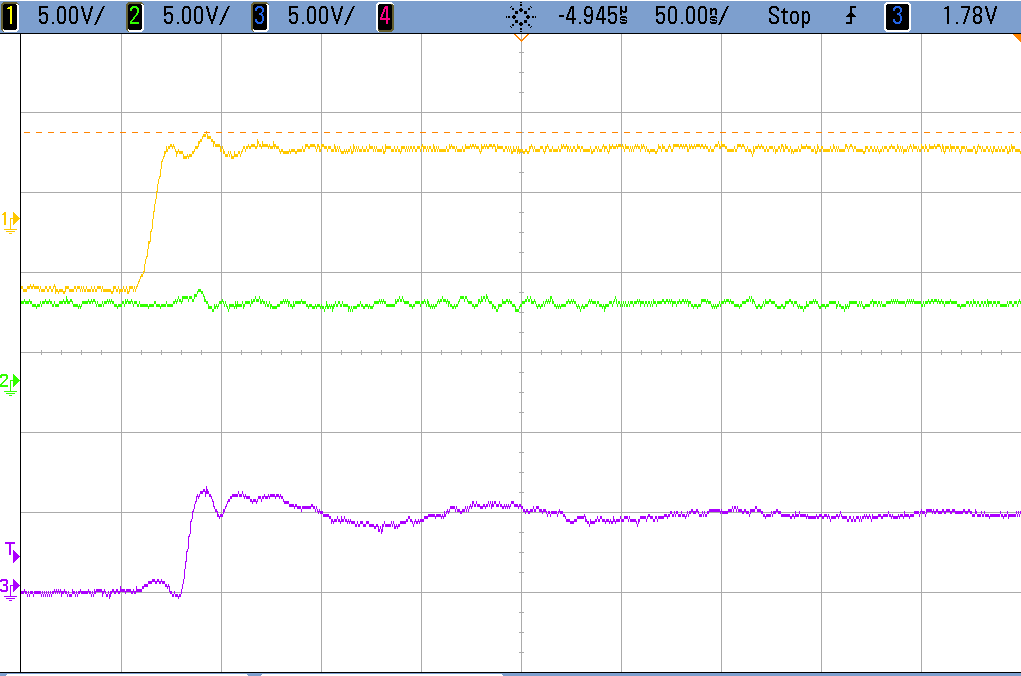
\includegraphics[width=0.5\textwidth]{../EJ6/Recursos/com_ffd_rise_osc} &
        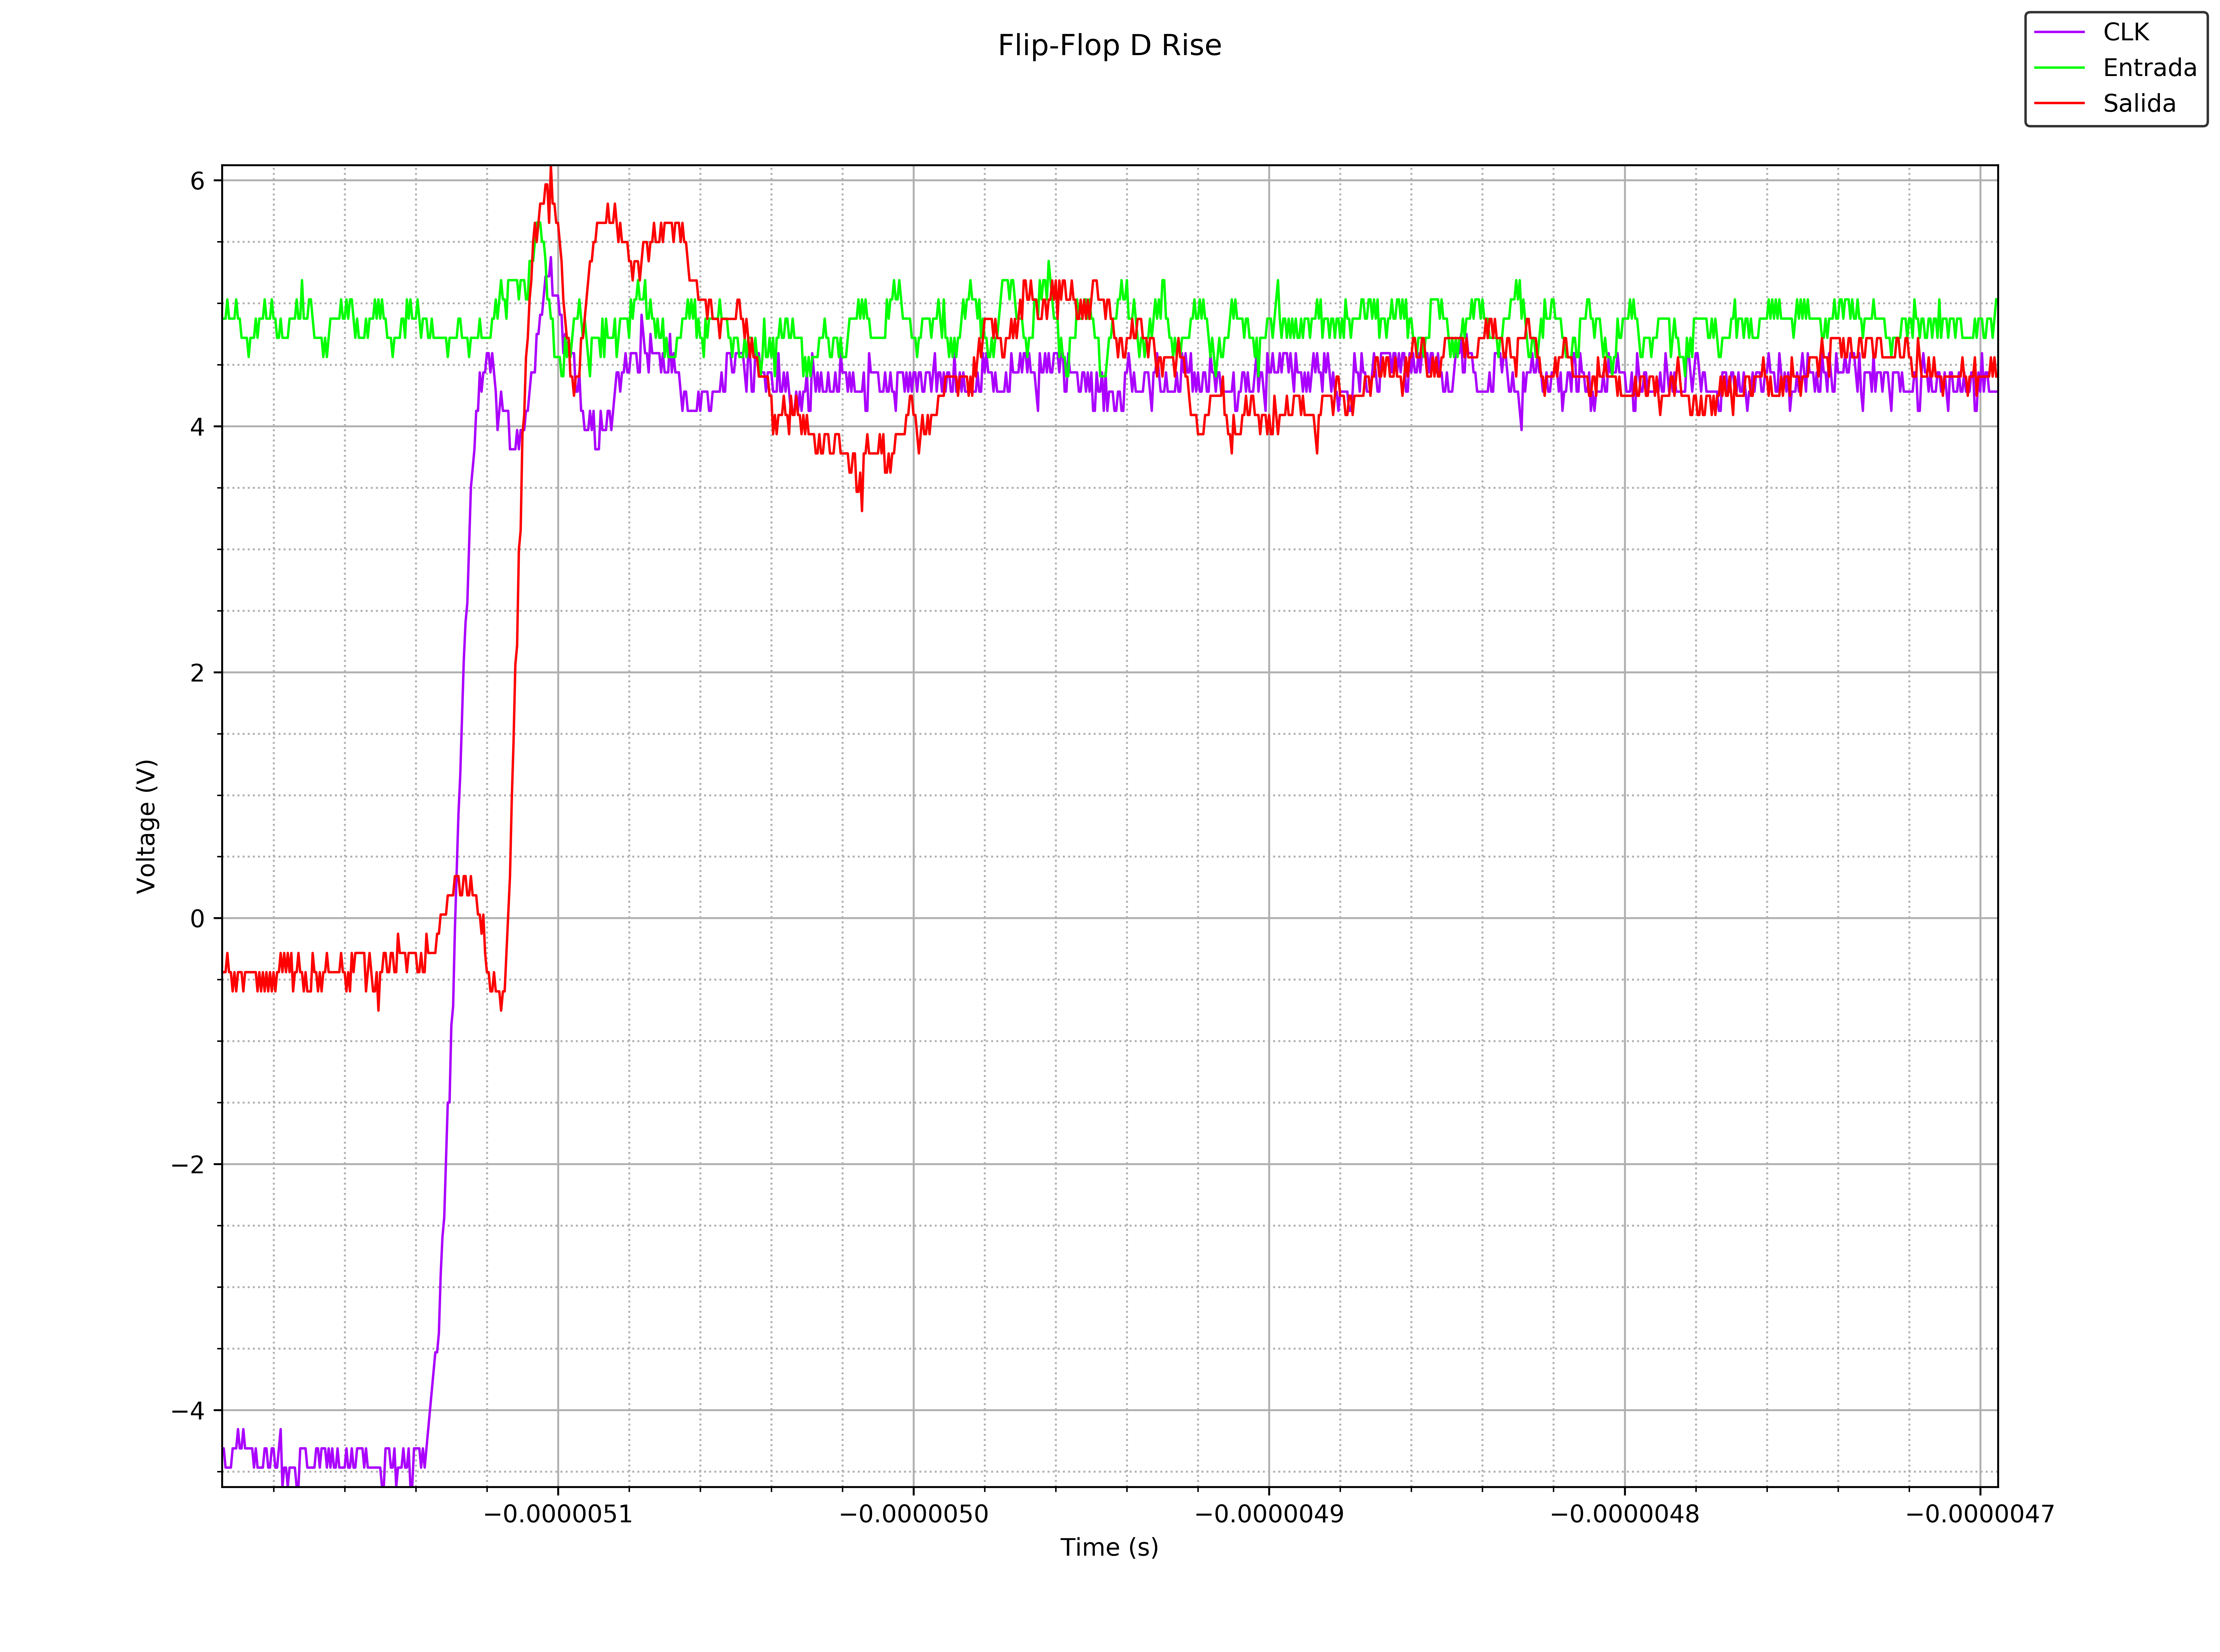
\includegraphics[width=0.5\textwidth]{../EJ6/Recursos/com_ffd_rise}
    \end{tabular}
    \caption{Transición del Flip-Flop D comercial de 0 a 1.}
    \label{fig:com_ffd_rise_ex6}
\end{figure}

\begin{figure}[H]
    \centering
    \begin{tabular}{c c}
        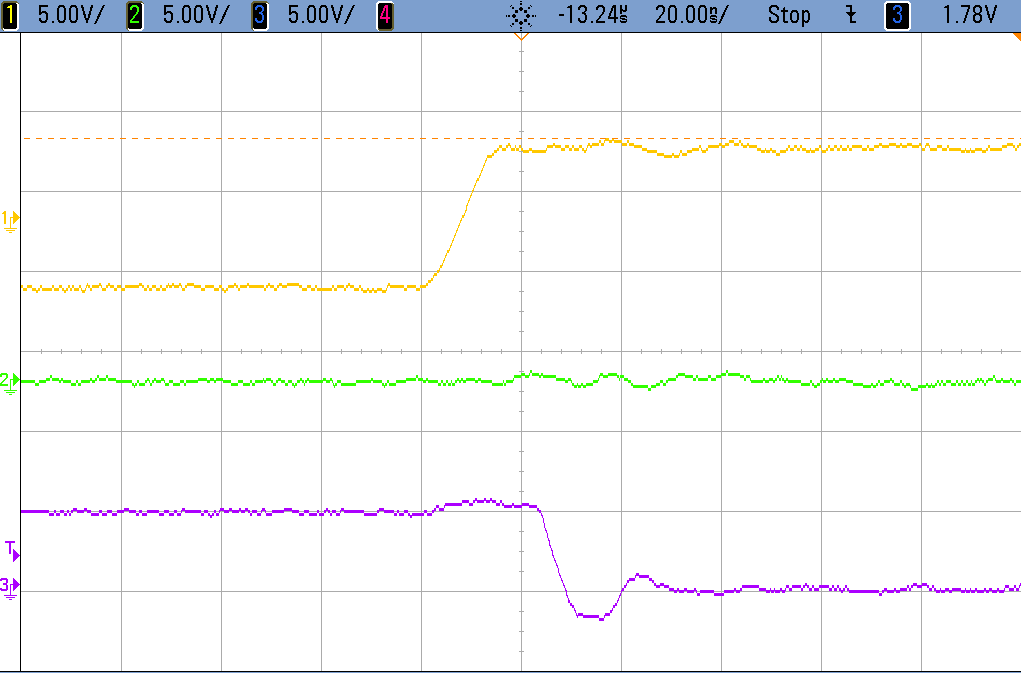
\includegraphics[width=0.5\textwidth]{../EJ6/Recursos/com_ffd_fall_osc} &
        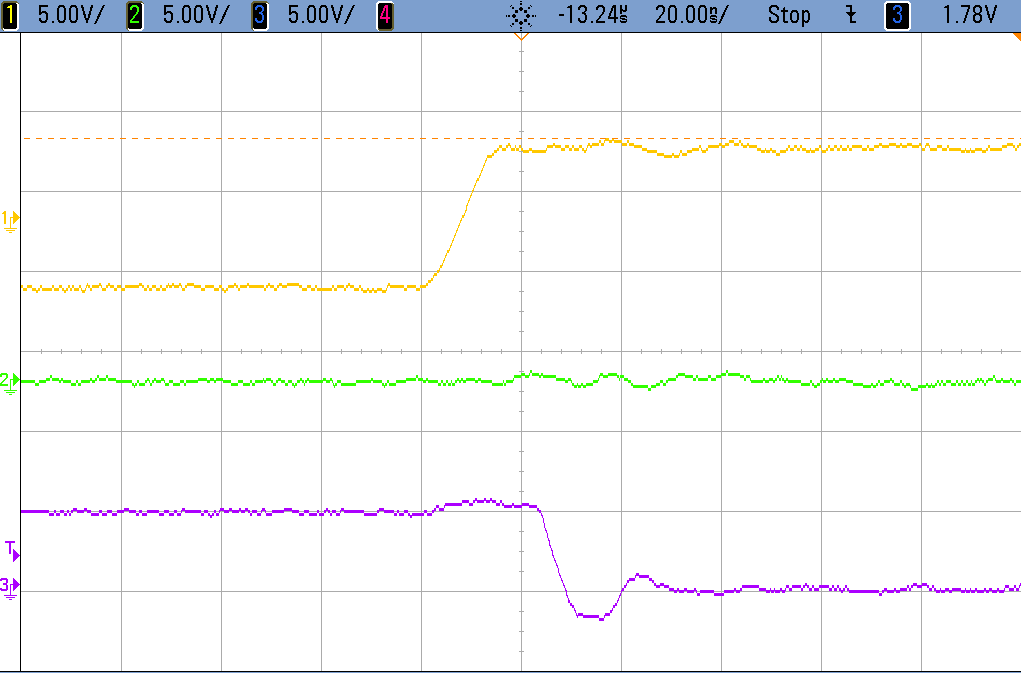
\includegraphics[width=0.5\textwidth]{../EJ6/Recursos/com_ffd_fall}
    \end{tabular}
    \caption{Transición del Flip-Flop D comercial de 1 a 0.}
    \label{fig:com_ffd_fall_ex6}
\end{figure}

Utilizando mediciones como las de la figura \ref{fig:ffd_ex6}, y teniendo en cuenta las definiciones de tiempo de set up y hold explicadas en secciones anteriores, se 
llega a medir estos parámetros para este Flip-Flop D.
Se dió, al igual que con los tiempos de rise y fall, que estos se encontraban cercanos a los 5ns, en el orden del límite impuesto por el osciloscopio, tanto para el armado 
con compuertas como el comercial.
Esto último también coincide con los mínimos de la hoja de datos, que los ubican en 5 y 15ns para hold y set up, respectivamente.\\
Finalmente, en el Flip-Flop también se aprecian transitorios de segundo orden, con frecuencias de aproximadamente 50MHz, tanto para el comercial como el de compuertas.
Nuevamente, la señal se puede considerar estable una vez transcurridos 3 períodos.



\subsubsection{Conclusión}
Se concluye resaltando el hecho de haber podido diseñar e implementar circuitos con compuertas lógicas cuyo comportamiento es el esperado, y sus parámetros 
característicos son comparables a aquellos de componentes comerciales.
En todos los casos, la respuesta del componente integrado se considera mejor, pero no se debe dejar de destacar que los valores del circuito armado se encuentran incluso 
dentro de los márgenes impuestos por las hojas de datos de los comerciales.